\label{desenvolvimento}

Esta parte do trabalho é dedicada à descrição da execução do procedimento metodológico. Aqui, descreve-se todo o desenvolvimento do trabalho, com o máximo de detalhes possível, desde a obtenção dos dados, até a coleta e análise dos resultados. A intenção final desta seção é descrever uma receita, que se seguida passo a passo, o resultado obtido será equivalente aos resultado deste trabalho.

\section{Busca e captura de dados para treinamento}

A primeira parte do desenvolvimento da proposta envolve todo o esforço de pesquisa, verificação e download de dados para que o modelo possa ser treinado. O modelo em questão será treinado e trabalhará com imagens portanto devemos encontrar e analisar bases de dados de imagens que se encaixem no escopo proposto. As imagens precisam ser imagens médicas e astronômicas, os dois grupos de imagens para os quais o modelo irá se especializar.

Encontrar imagens que se encaixem nas descrições acima, não é nada trabalhoso com os motores de busca disponíveis na internet. Contudo, encontrar uma quantidade grande de imagens consistentes não é uma tarefa tão simples. Por imagens consistentes, refiro a um conjunto de imagens:

\begin{enumerate}
    \item que seja composto por imagens de resoluções próximas ou uniformes. Os modelos são preparados para treinarem e serem alimentados com imagens de uma dimensão constante, ou seja, para os treinar com imagens de uma resolução de 256 \textit{pixels} de altura por 256 \textit{pixels} de largura, deve ser garantido que todo o restante da base de imagens esteja nesta resolução. Alguns modelos aceitam treinar com resoluções heterogêneas (i. e. as resoluções diferem de imagem pra imagem) desde que a largura e a altura sejam divisíveis por um número definido \textit{N}.

    \item que possua um número de imagens suficiente para um treinamento significativo. Este requisito apesar de não ser exato, é extremamente importante para a qualidade dos resultados. Com poucas imagens de treinamento, o modelo não será capaz de aprender os padrões que descrevem aquele grupo de imagem e o resultado é pobre. No caso de redes adversárias geradoras, imagens visualmente e matematicamente distintas do objetivo podem ser geradas, se porventura os modelos forem treinados com dados insuficientes.
\end{enumerate}

Caso o primeiro requisito não seja cumprido, é possível, ainda que manualmente, uniformizar a resolução das imagens. O segundo tópico no entanto, é mais crítico, e caso não seja possível cumpri-lo, técnicas avançadas de gerações de bases de dados a partir de um conjunto de dados podem ser utilizadas, como foi mencionado na seção \ref{justificativa}. Apesar desta possibilidade existir, esta técnica foge do escopo do trabalho.

Como os objetivos do trabalho envolvem treinamento com imagens de áreas específicas, médicas e astronômicas, alguns recursos específicos para estas áreas podem ser úteis. Existem fontes formais de imagens médicas e imagens astronômicas. Alguns exemplos de fontes para imagens médicas são:

\begin{itemize}
    \item OpenNeuro \cite{openneuro_openneuro_2022}, antigo OpenfMRI \cite{openfmri_openfmri_2022}. Site com diversas bases de dados contendo imagens médicas. Entre elas, bases de imagens de ressonância magnética.
    \item FastMRI \cite{fastmri_fastmri_2022}. Site com imagens de ressonância magnética.
    \item \textit{Cancer Image Archive} \cite{cancer_imaging_archive_cancer_2022}. Serviço de banco de imagens médicas sobre câncer.
\end{itemize}

E também, alguns exemplos de bases de imagens astronômicas:

\begin{itemize}
    \item Kaggle \cite{srivastava_astronomy_2024}. O Kaggle em si, é uma comunidade de ciência de dados e possui diversos dados e recursos para treinamento de modelos de aprendizado de máquina. 
    \item SDSS \cite{sdss_sloan_2024}. O SDSS (Sloan Digital Sky Survey) regularmente publica e atualiza bases de dados de imagens de astros e objetos profundos no espaço.
\end{itemize}

Nas subseções abaixo, está descrito o procedimento utilizado para acessar as bases de dados médicas e astronômicas, começando pelas imagens médicas, as mais trabalhosas de se encontrar.

\subsection{Obtenção de imagens médicas}
\label{sec:imagens_medicas}

Encontrar imagens médicas individuais ou até grupos pequenos, com até 300 exemplos, foi uma tarefa simples. Como salientado anteriormente, os mecanismos de busca modernos nos permitem fazer tal busca com precisão e velocidade. Todavia, encontrar uma base de dados com alguns milhares de imagens não foi simples nem rápido.

Algumas bases de dados com quantidades grandes de exemplares foram encontradas nos serviços citados. No entanto uma prioridade baixa foi atribuída a estas, devido principalmente aos problemas de resoluções de imagens. Ou as resoluções eram muito baixas ou eram muito heterogêneas, e apesar de ser possível ajustar isso posteriormente, é um trabalho extra a ser evitado.

Um serviço particularmente interessante para o caso de uso estudado, é o \textit{Cancer Image Archive} \cite{cancer_imaging_archive_cancer_2022} (figura \ref{fig:fig14}). Neste serviço, é possível buscar as bases de imagens separadas por coleções classificadas por diversos aspectos como tipo de equipamento que produziu a imagem, tipo de câncer do qual as imagens se tratam, data de atualização dos dados, espécie da qual as imagens se tratam, entre outros. Grandes bases de dados foram encontradas utilizando este serviço, algumas com centenas de gigabytes de imagens.

\begin{figure}[H]
    \centering
    \caption{Captura de tela da página principal do \textit{Cancer Imaging Archive}.}
    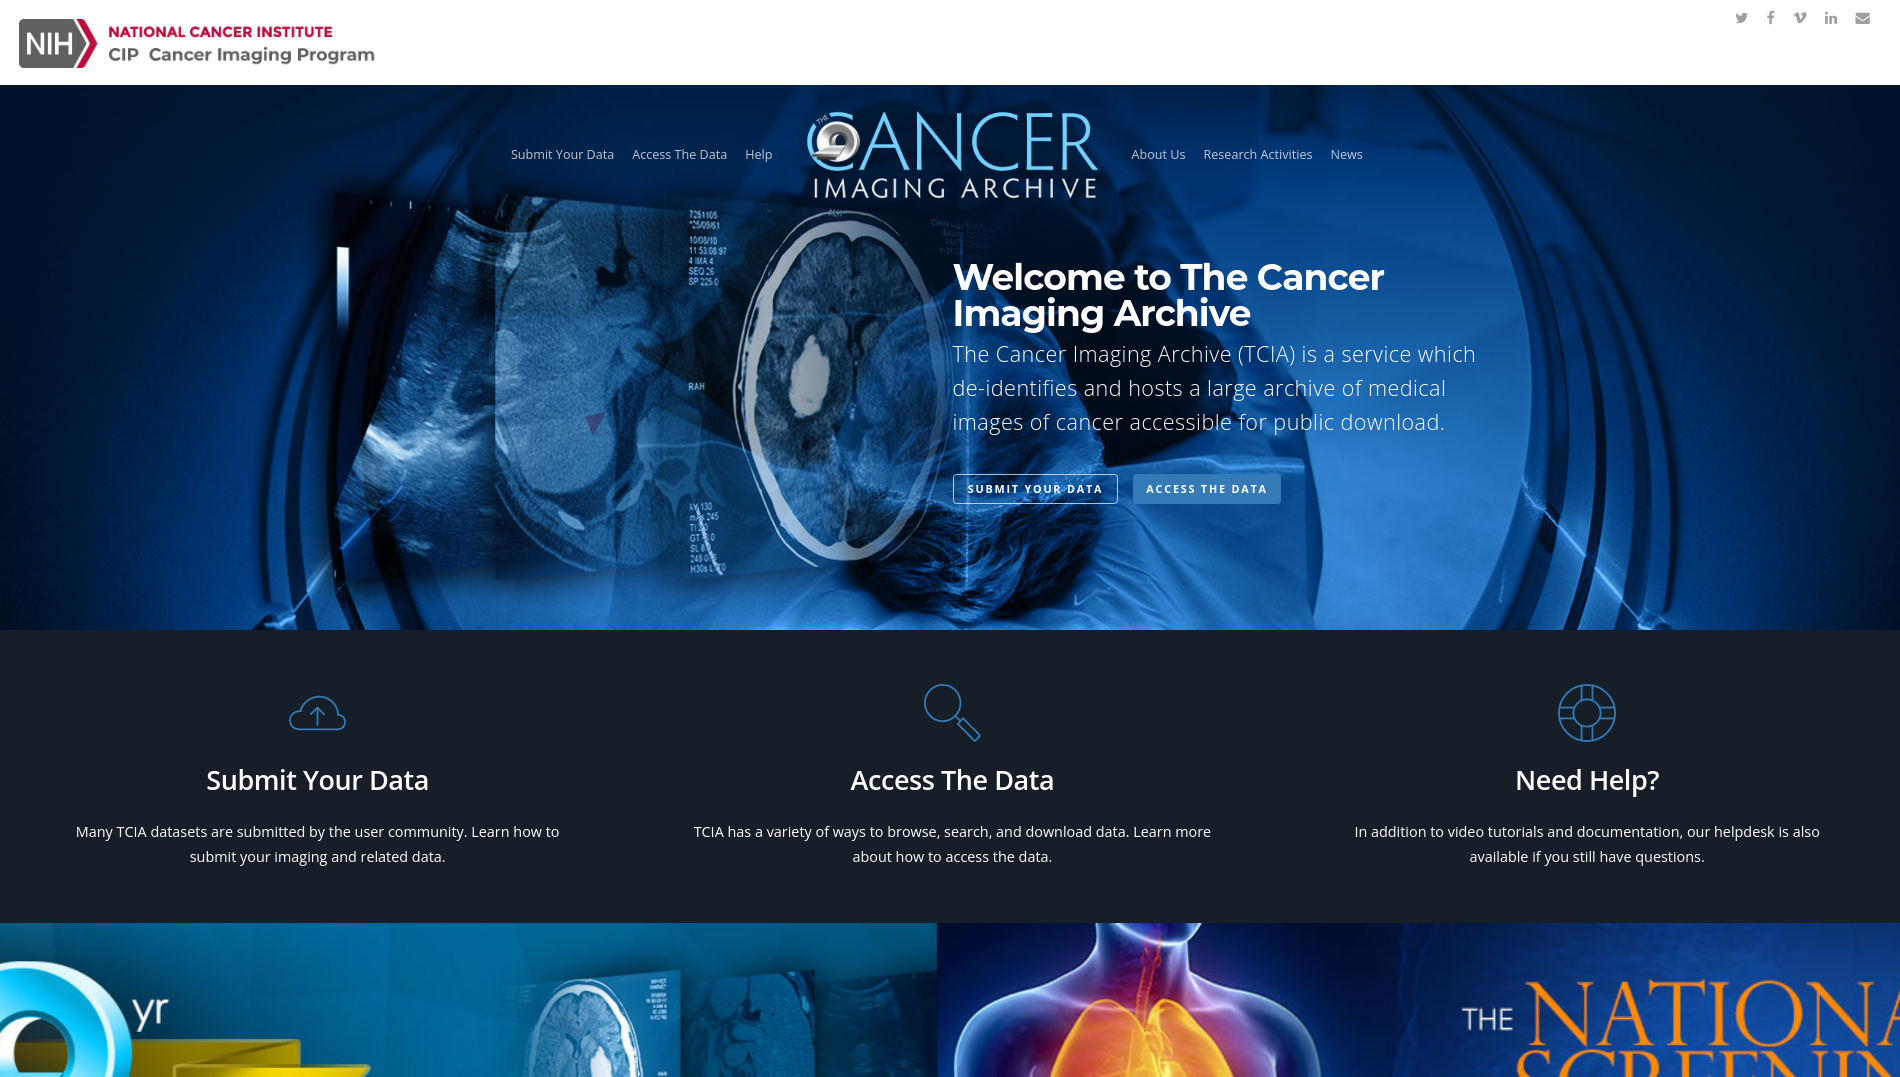
\includegraphics[width=13cm]{fig/cancer_imaging_archive.png}
    \legend{Fonte: \cite{cancer_imaging_archive_cancer_2022}}
    \label{fig:fig14}
\end{figure}

A base de dados escolhida foi a base de imagens de câncer de mama \textit{Duke Breast Cancer MRI} \cite{saha_machine_2018} por mera tentativa e erro. Após procurar por algumas coleções, este conjunto de imagens é interessante por alguns motivos:

\begin{itemize}
    \item Possui uma quantia significativa de imagens: 773126. Por motivos de armazenamento, apenas uma fração da base de imagens foi utilizada;
    \item As imagens escolhidas da coleção possuem resoluções uniformes, ou pelo menos aproximadas. Apenas parte da base foi utilizada, por isso, o termo "escolhidas". Isso não é um problema pois a base de dados contém tantas imagens, que a quantia total é impraticável para o escopo do trabalho. As imagens ocuparam cerca de 370GB em disco após o download. 
    
\end{itemize}

Uma peculiaridade deste serviço utilizado, é a existência de uma ferramenta oficial para baixar as imagens chamada \textit{NBIA Data Retriever} \cite{cancer_imaging_archive_cancer_2022}(Vide figura \ref{fig:fig15}). Nem todas as bases de dados requerem o download pela ferramenta mas a base de dados escolhida só estava disponível por este método.

\begin{figure}[H]
    \centering
    \caption{Captura de tela do \textit{NBIA data retriever}.}
    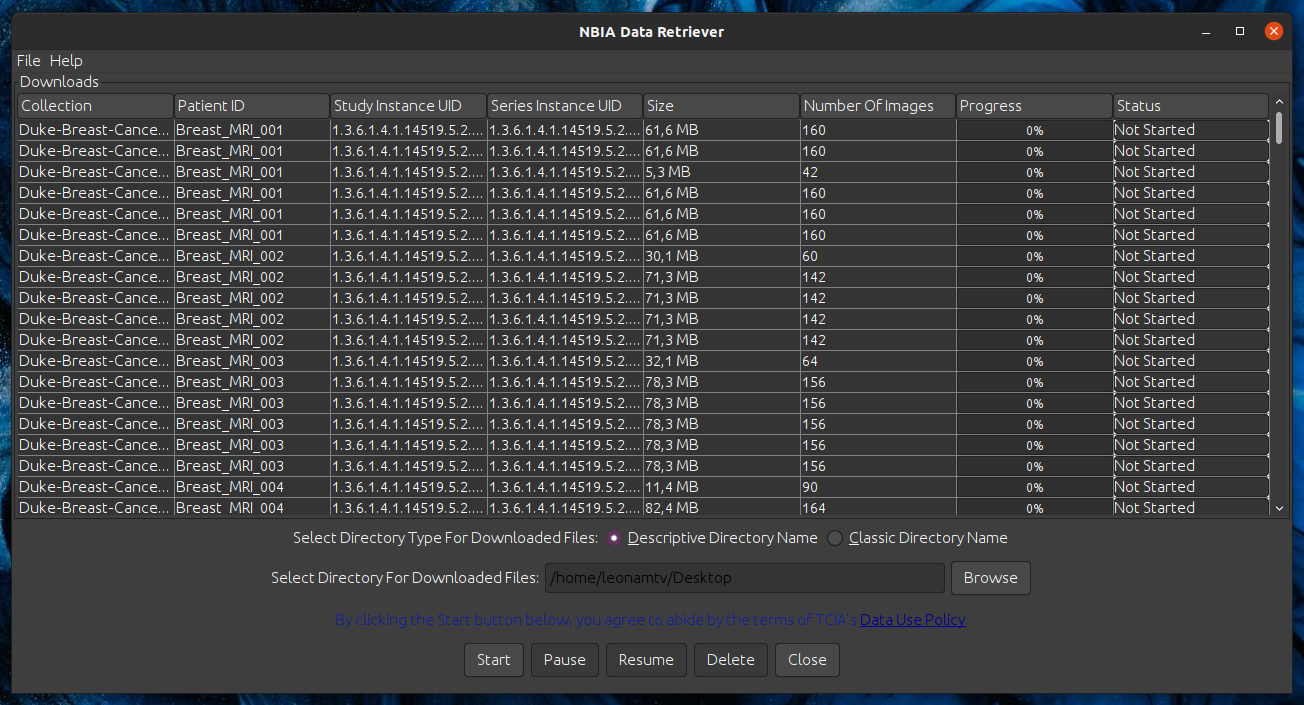
\includegraphics[width=13cm]{fig/nbia_data_retriever.png}
    \legend{Fonte: Captura de tela tirada pelo autor.}
    \label{fig:fig15}
\end{figure}

O procedimento para fazer o download segue os passos abaixo:

\begin{enumerate}
    \item Deve-se criar uma conta no site \cite{cancer_imaging_archive_cancer_2022} (figura \ref{fig:fig14}) para ter acesso ao \textit{carrinho};

    \item Adicione as bases de dados de interesse no carrinho e faça o download;

    \item Um arquivo com o nome no formato \textbf{manifest-xxx.tcia} será baixado. Este arquivo contém todas as informações que o software \textit{NBIA Data Retriever} (figura \ref{fig:fig15}) precisa para fazer o download das imagens;

    \item Instale o programa \textit{NBIA Data Retriever} (figura \ref{fig:fig15}) e abra o arquivo baixado com ele;

    \item Faça o download das imagens.
\end{enumerate}

\subsection{Obtenção de imagens astronômicas}
\label{sec:imagens_astronomicas}

Diferente das imagens médicas, encontrar a base de dados de astronomia foi uma tarefa objetiva. Logo nas primeiras tentativas, é possível encontrar uma base de dados que se encaixe nos requisitos, com pouco esforço de pesquisa.

A base de dados astronômica encontrada, possui imagens de baixa resolução no geral. Por volta de 258 pixeis de largura e altura. Apesar de a qualidade visual das imagens serem pobres, a baixa resolução traz menos estresse para os recursos computacionais disponíveis para treinamento.

Diferente da base de dados anterior que é monocromática, esta é colorida. Tal complexidade afeta o desempenho do treinamento dos modelos. Vide seção \ref{sec:desenvolvimento:general-considerations-post-processed-images}

\section{Preparação das imagens para treinamento}
\label{sec:prep-imgs}

As imagens encontradas não estavam integralmente prontas para o treinamento. Processamento anterior à esta fase é necessário para poder realizá-la com sucesso. Os modelos possuem entradas com formatos e resoluções específicos e treiná-los requer atenção à tais especificações.

O modelo em questão, na forma como foi implementado possui alguns requisitos ou recomendações sobre como deve ser treinado:

\begin{itemize}
    \item As imagens devem possuir uma resolução uniforme. Mesma largura e mesma altura para todo o conjunto de imagens;

    \item A resolução das imagens deve ser divisível por 4. Este é um requisito específico para a ESRGAN de super-resolução em 4 vezes;

    \item As imagens devem estar em um formato capaz de ser lido pelas camadas de entradas do modelo (qualquer formato amplamente utilizado é aceitável e.g. png, jpg etc.).
\end{itemize}

A resolução das imagens estava de acordo com os requerimentos. Os bancos de imagens já proveram as imagens com uma resolução uniforme entre todas os exemplares. Contudo, por limitações de recursos, há possibilidades de as imagens serem muito grandes para o treinamento. O modelo é treinado em grupos de imagens. Estes grupos possuem uma quantidade fixa de exemplares escolhidos aleatoriamente pelo modelo a partir de uma base de treinamentos e esta quantidade é definida através de um parâmetro chamado \textit{batch size}. Por exemplo, se a base de dados contém 6000 imagens e um \textit{batch size} de 60 é utilizado, o treinamento do modelo irá ocorrer de 60 em 60 imagens escolhidas aleatoriamente dentro das 6000 imagens disponíveis. Este parâmetro é particularmente interessante para-se regular a quantidade de imagens em memória simultaneamente durante toda a fase de treinamentos. Quanto mais imagens na memória ao mesmo tempo, mais rápido será o treinamento pois menos leituras de disco serão realizadas.

Antes do treinamento definitivo, uma série de escolhas devem ser tomadas, para que o tempo e os recursos para treinar o modelo caibam dentro do disponível. Pode-se reduzir a resolução das imagens para que seja possível colocar mais imagens na memória mas isso pode reduzir a qualidade do modelo final, já que reduzir a resolução nada mais é que reduzir a qualidade (e quantidade de detalhes) dos dados utilizados para treinamento. Menos qualidade (quantidade de detalhes), menos padrões para o modelo aprender e em consequência este produzirá resultados inferiores. Há também a possibilidade de se  reduzir o tamanho do \textit{batch size}. Essa ação no entanto, faz com que durante o treinamento, mais leituras em disco ocorram e isso prolonga consideravelmente o tempo de duração desta fase.

Como os recursos disponíveis são baixos e limitados, devo adotar uma combinação das alternativas apresentadas para treinar o modelo. É então necessário, reduzir a resolução das imagens até uma resolução onde detalhes ainda são suficientes para um aprendizado significativo. A redução do \textit{batch size}, para a não violação do limite de memória, é também uma alternativa adotada.

\subsection{Conversão de imagens médicas para um formato comum}
\index{DICOM}

Para treinar o modelo, as imagens utilizadas precisam estar em um formato comum, como mencionado anteriormente. As imagens médicas no entanto, estão em um formato especial utilizado internacionalmente em contexto médico: o formato \textit{DICOM} (arquivos com extensão ".dcm"). \textit{DICOM} é um padrão internacional de imagens médicas. É o padrão para armazenar, transmitir e utilizar imagens médicas de forma digital. O nome é sigla para \textit{Digital Imaging and Communications in Medicine} (Imagem e comunicação digital em medicina, do inglês). O formato revolucionou a forma como equipamentos de imagem funcionavam desde que foi desenvolvido. \cite{dicom_standard_history_2019, medical_connections_dicomobjects_2011, dicom_standard_current_2024, medical_connections_dicom_2007, weston_understanding_2020}
    
O padrão \textit{DICOM} é complexo e longo e não cabe ao escopo deste trabalho descrever em detalhes o seu funcionamento e implementações. Felizmente, este padrão é amplamente utilizado na medicina e há bastante documentação esclarecendo tudo aquilo que que o progresso do trabalho exige.

As imagens médicas que serão utilizadas para o treinamento estão todas neste formato e precisam ser convertidas para um formato aceito pelo modelo. Primeiramente, tal conversão deve ser realizada de forma automatizada, dada tamanha a quantidade de imagens.

Encontrar uma biblioteca capaz de extrair informações de imagens \textit{DICOM} é uma tarefa simples, dada a popularidade deste padrão na comunidade técnica. Imagens deste formato armazenam muito mais que apenas informações sobre a localização e cores dos pixeis que formam a imagem. Informações sobre o paciente e sobre o local onde a imagem foi capturada ficam contidos também no arquivo, desta forma as imagens sempre carregam informações sobre suas origens: onde foram geradas e de quem é o corpo descrito por aquela imagem.

É possível acessar estas informações com a biblioteca \textit{pydicom} \cite{pydicom_pydicom_2022} para \textit{python}. Vide código abaixo:

\begin{figure}[H]
    \centering
    \caption{Código para imprimir informações de um arquivo \textit{DICOM}.}
    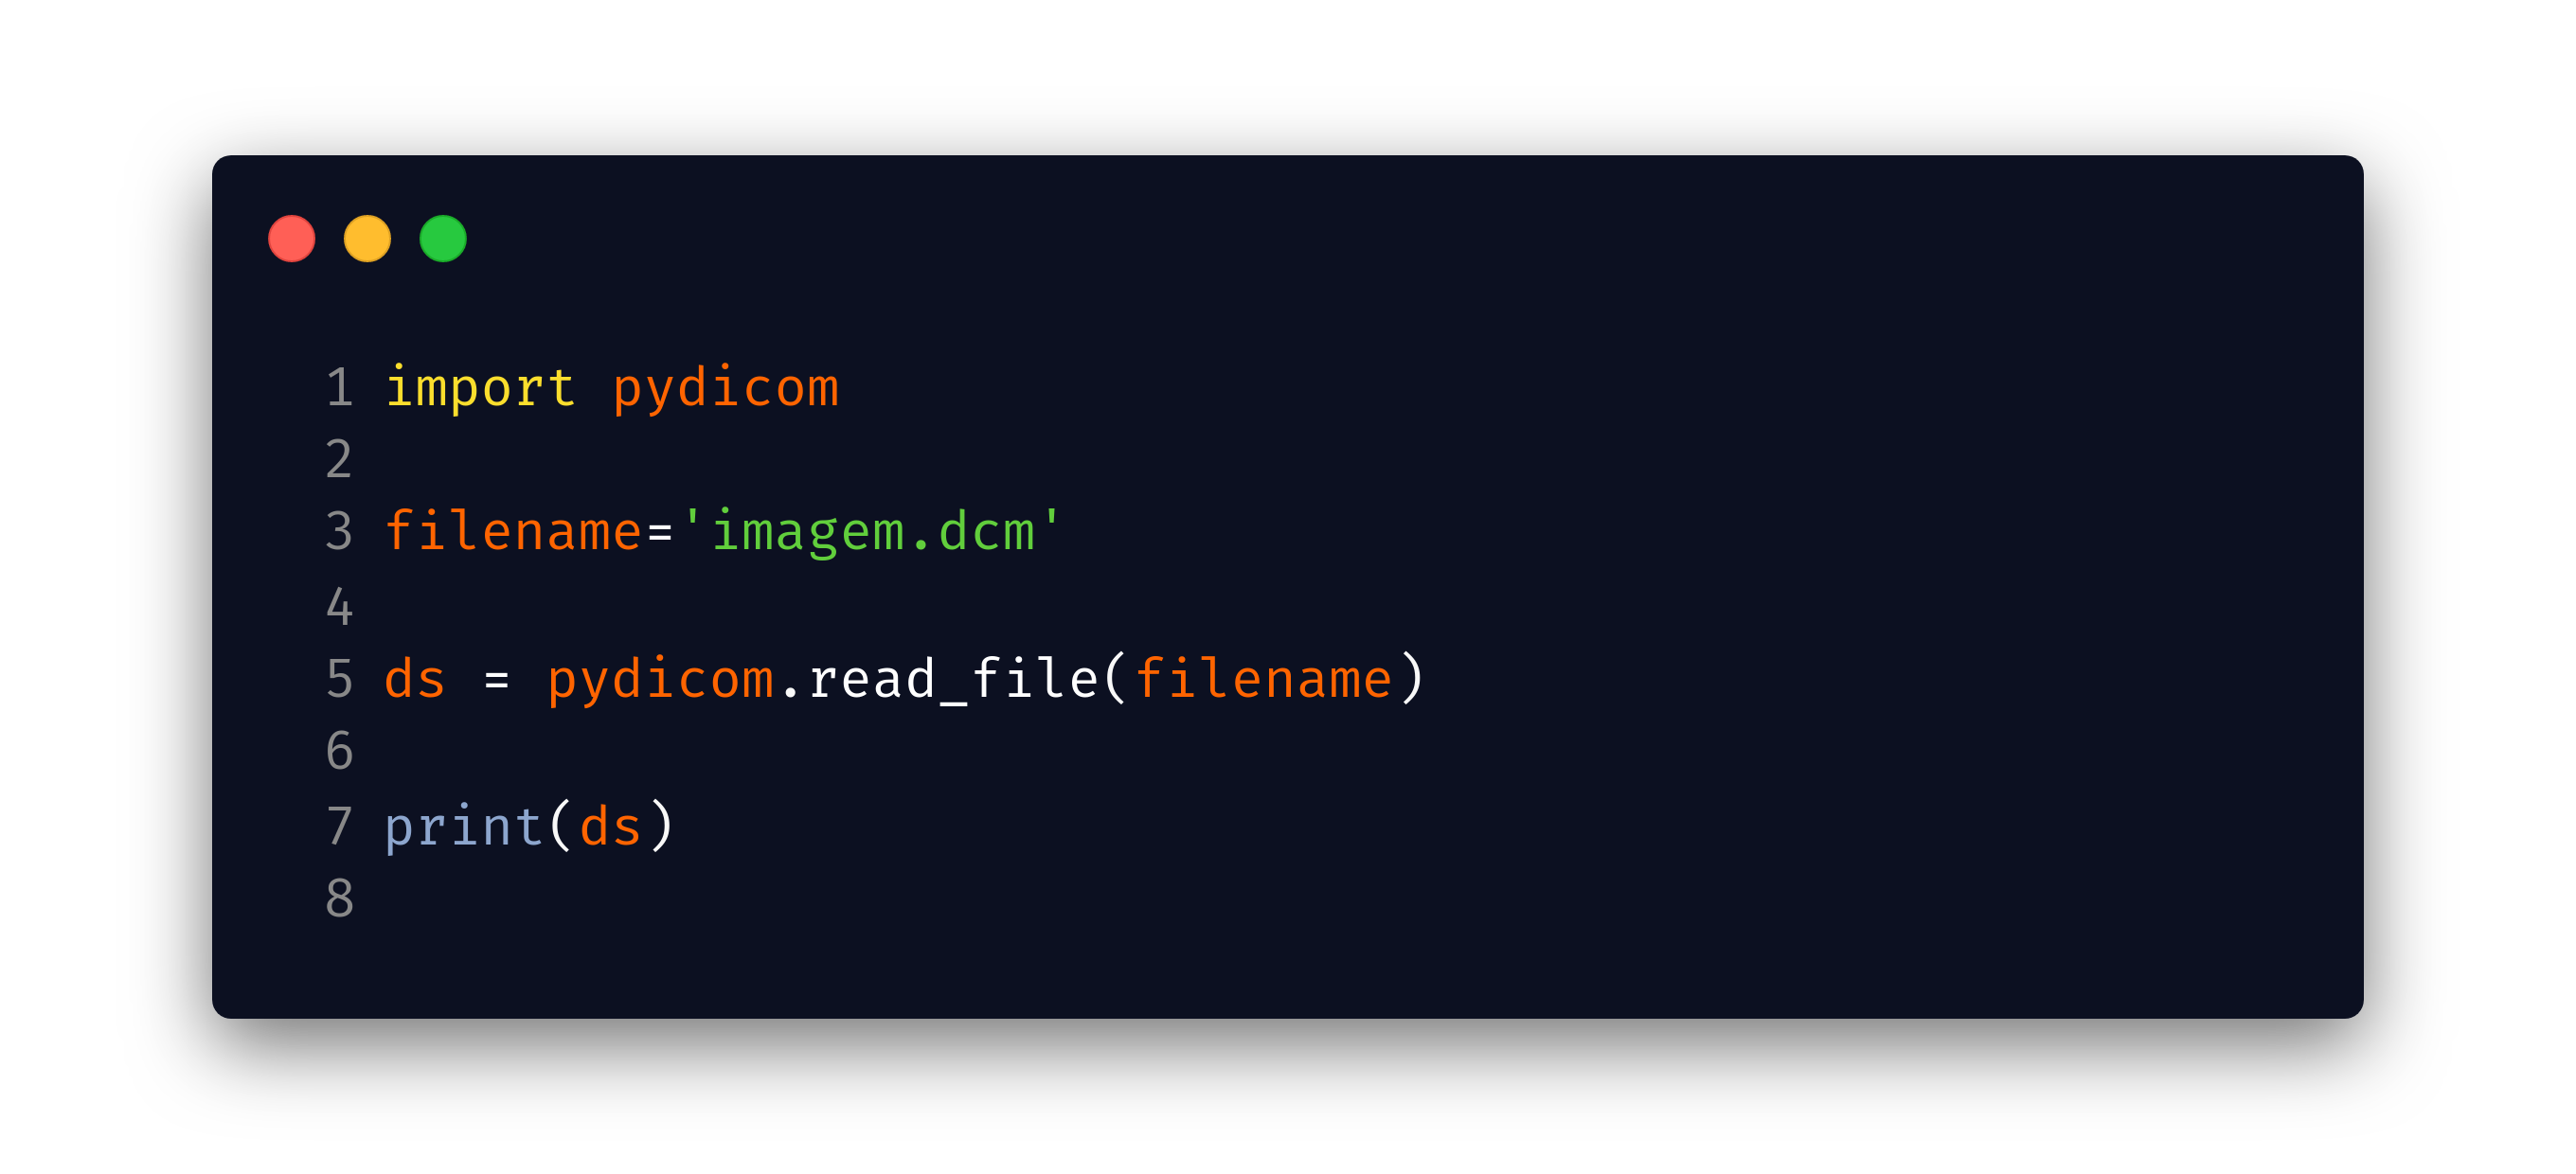
\includegraphics[width=14cm]{fig/code_1.png}
    \legend{Fonte: Autor.}
    \label{fig:fig16}
\end{figure}

O código da imagem \ref{fig:fig16} acima, produz a seguinte saída:

\begin{figure}[H]
    \centering
    \caption{Saída obtida com a execução do código contido na imagem \ref{fig:fig16}.}
    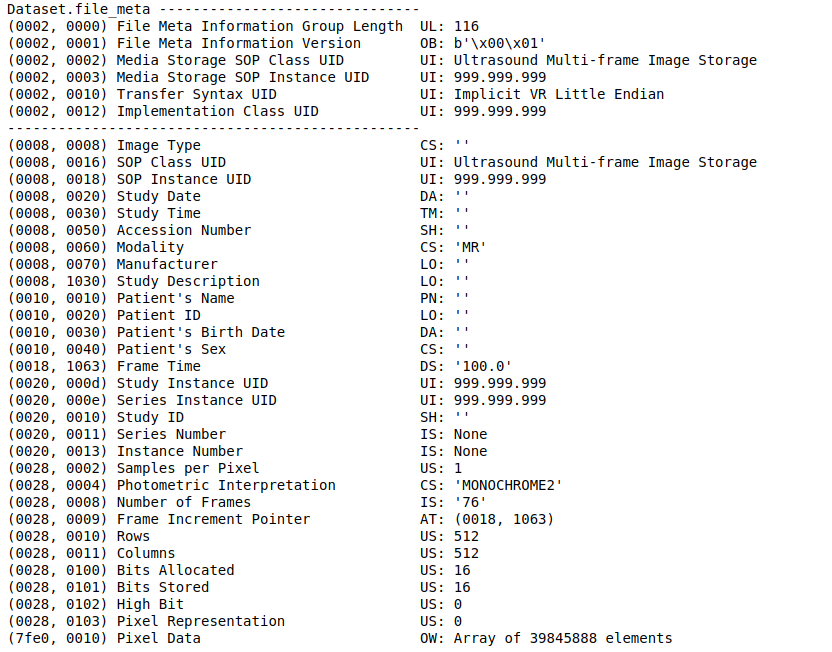
\includegraphics[width=12cm]{fig/output_1.png}
    \legend{Fonte: Autor.}
    \label{fig:saida:fig16}
\end{figure}

De acordo com a saída, o arquivo \textit{DICOM} utilizado traz uma série de informações relevantes para o contexto medicinal. Para o objetivo deste trabalho, o interesse é voltado apenas ao conteúdo do campo \textit{Pixel Data} (vide imagem \ref{fig:fig17}).

\begin{figure}[H]
    \centering
    \caption{Saída obtida com a execução do código contido na imagem  \ref{fig:fig16}, destacando o campo de interesse.}
    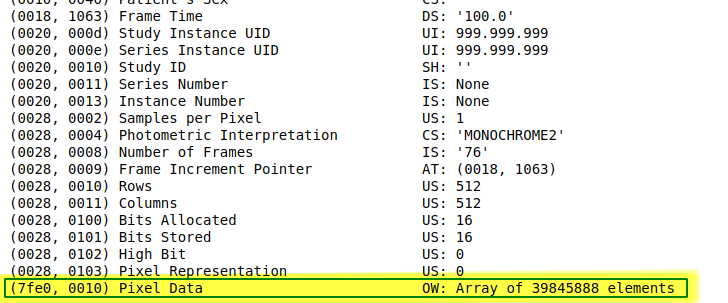
\includegraphics[width=12cm]{fig/output_1_v2.png}
    \legend{Fonte: Autor.}
    \label{fig:fig17}
\end{figure}

Este atributo contém as informações da imagem em si. Neste objeto há tudo que é necessário para converter as imagens em um formato comum. Com algumas bibliotecas auxiliares, estes dados podem ser inseridos em uma estrutura de dados auxiliar, através das quais as imagens são escritas em um formato específico, como \textit{jpg} por exemplo. O código abaixo, faz justamente isso.

\begin{figure}[H]
    \centering
    \caption{Código para converter uma imagem \textit{DICOM} para o formato \textit{jpg}.}
    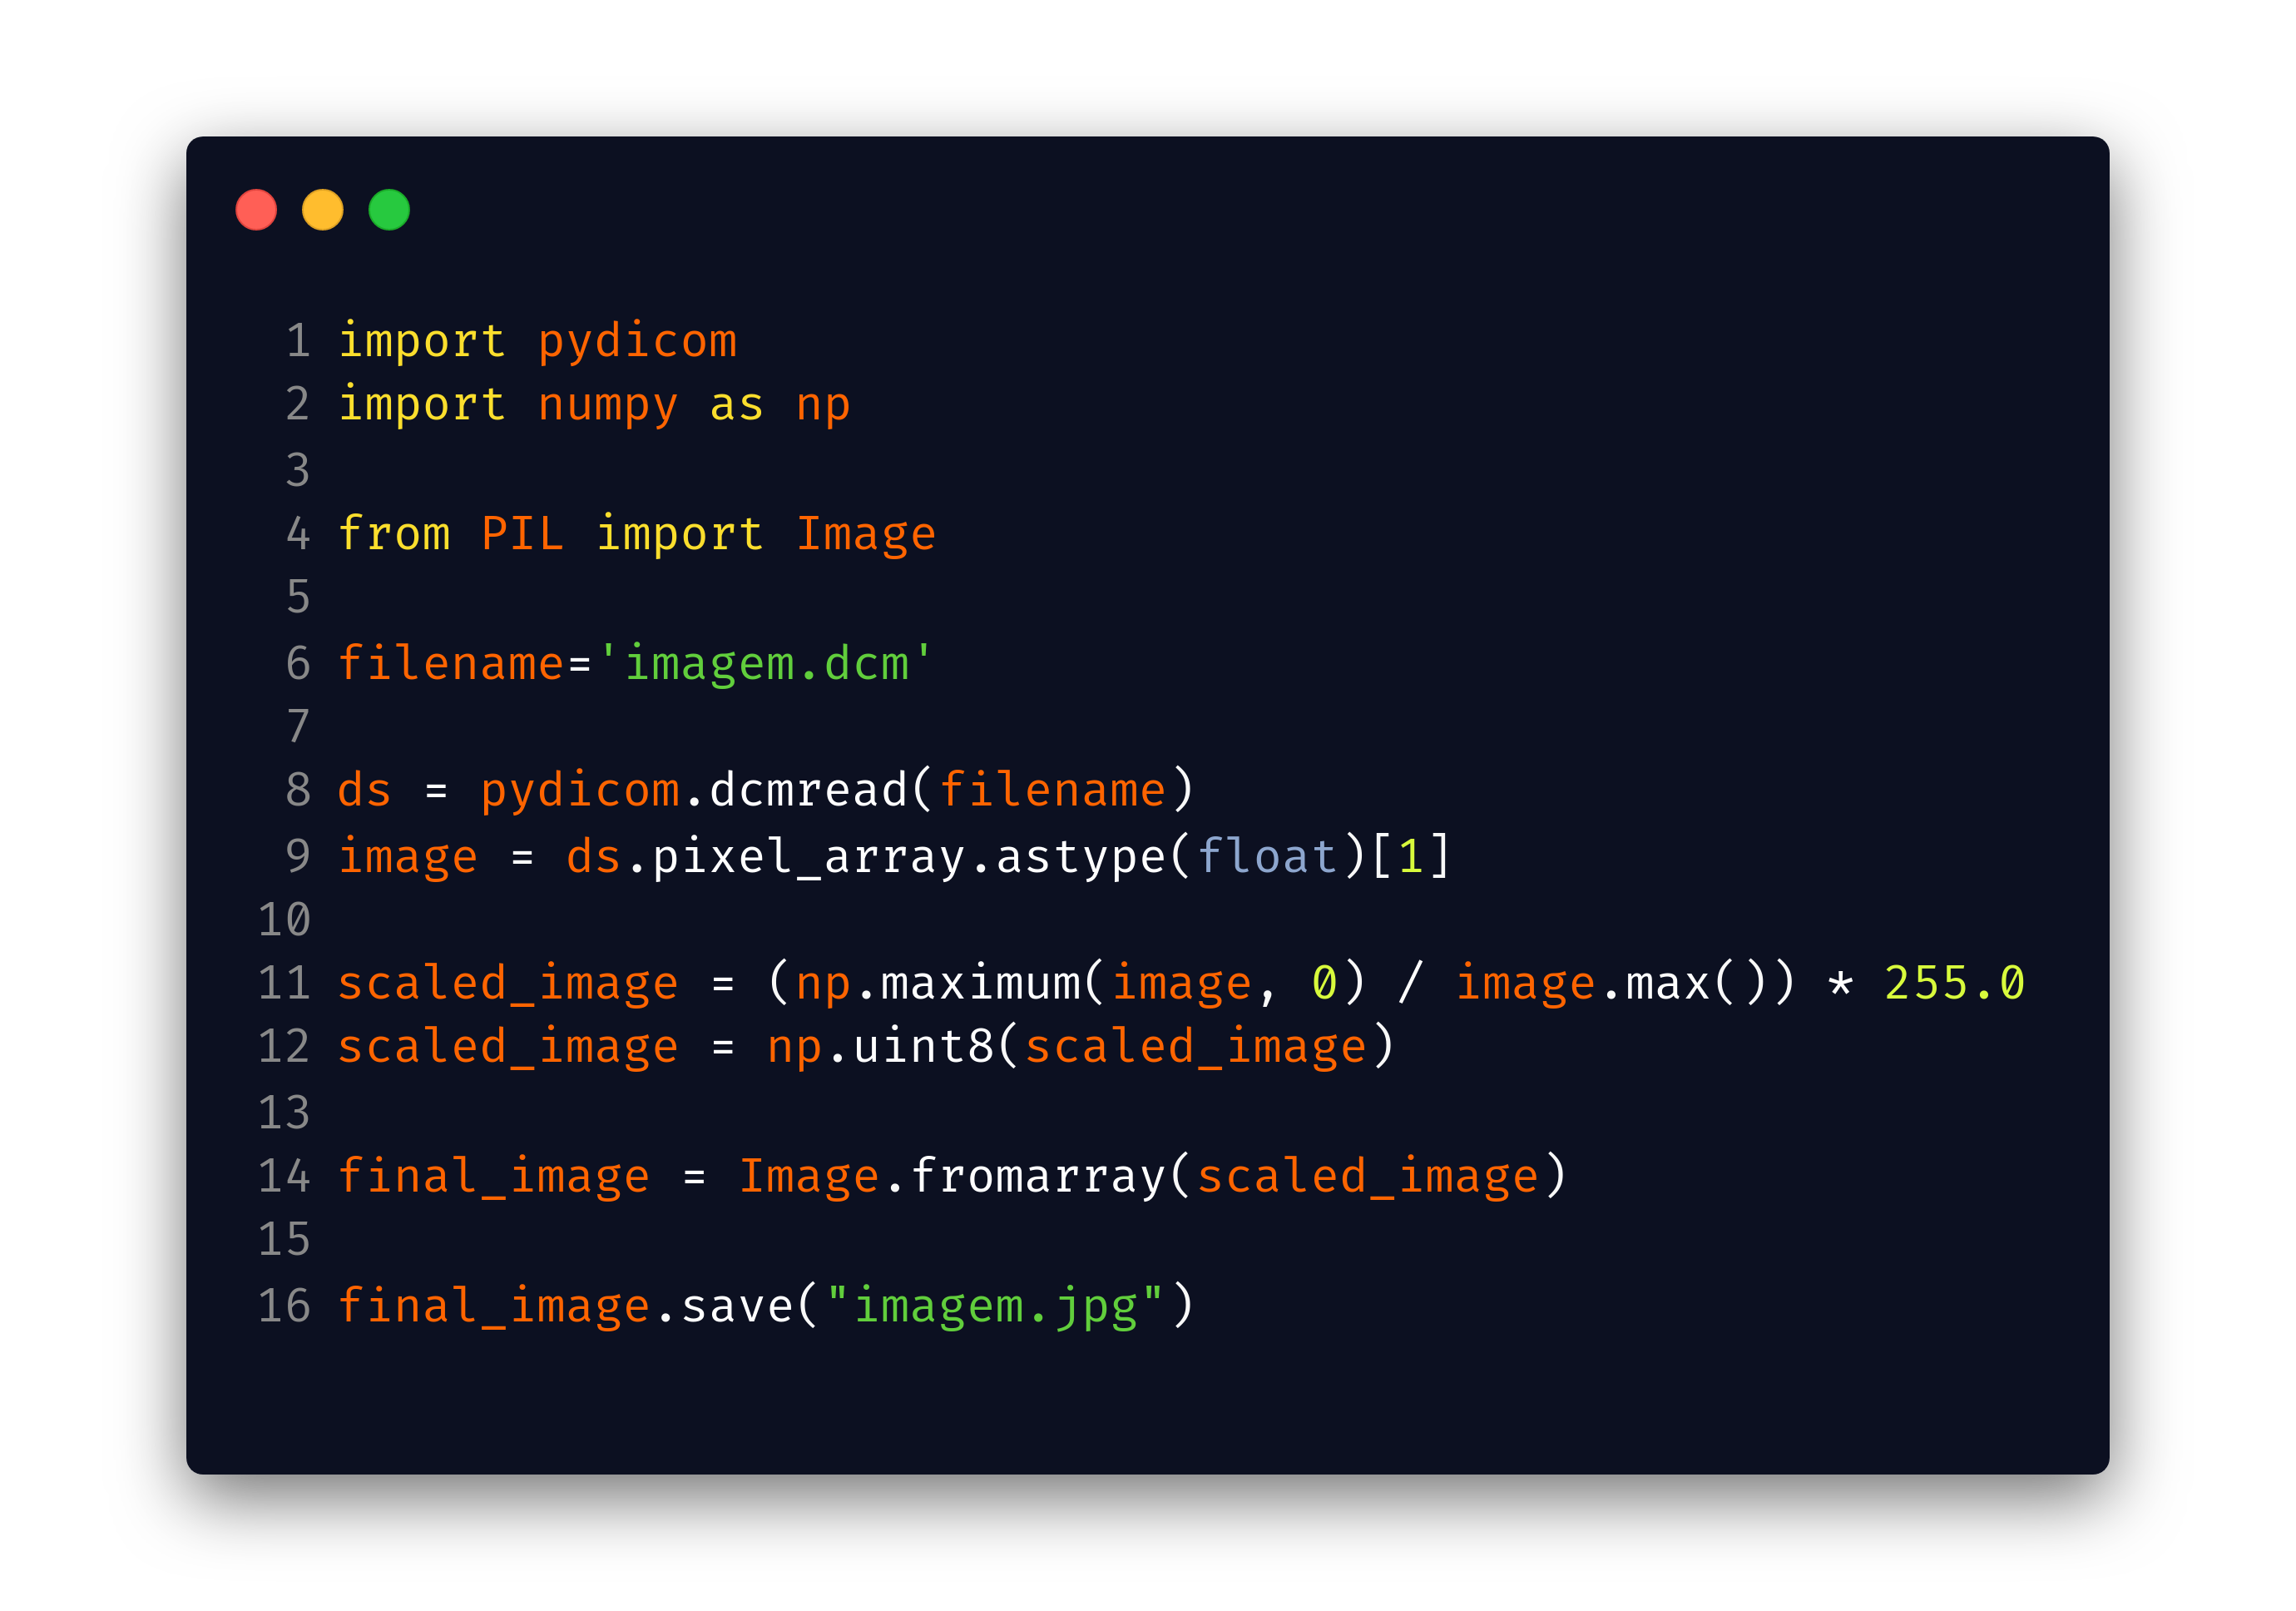
\includegraphics[width=12cm]{fig/code_2.png}
    \legend{Fonte: Autor.}
    \label{fig:fig18}
\end{figure}

Alguns detalhes sobre o código contido na imagem \ref{fig:fig18} valem uma descrição e explicação, dada sua importância para que a conversão seja feita com sucesso.

Na linha 9, o programa lê o arquivo de imagem como números de ponto flutuante e no final da linha, captura o item na segunda posição (posição 1, já que o índice em \textit{python} se inicia em zero). Este detalhe é de extrema importância pois os arquivos \textit{DICOM}, podem conter mais de uma imagem por arquivo. As imagens contidas em um arquivo \textit{DICOM} possuem mesma largura e altura, e são indexadas por imagem individual, como mostra a imagem abaixo:

\begin{figure}[H]
    \centering
    \caption{Estrutura de imagens \textit{DICOM}.}
    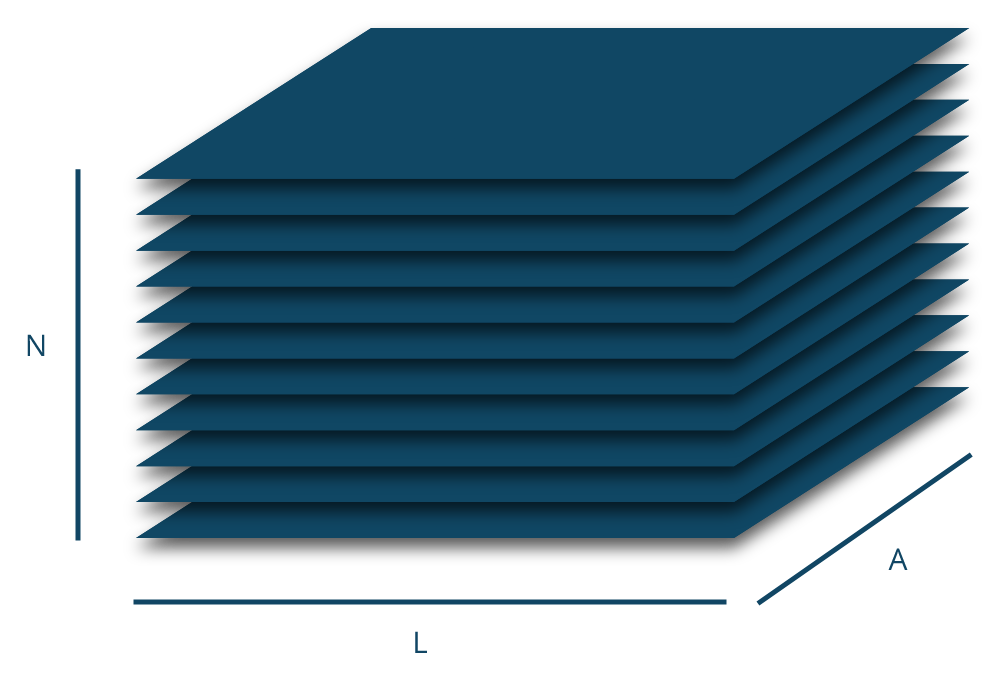
\includegraphics[width=9cm]{fig/dicom_img.png}
    \legend{Fonte: Autor.}
    \label{fig:fig19}
\end{figure}

Na imagem \ref{fig:fig19}, \textit{L} representa a largura -- uniforme para todas as imagens; \textit{A} representa a altura -- também uniforme para todas as imagens -- e \textit{N}, o número de imagens contidas no arquivo. Este valor \textit{N} pode ser encontrado nos metadados do arquivo \textit{DICOM} em um atributo chamado \textit{Number of frames} como destacado na imagem \ref{fig:fig20}:

\begin{figure}[H]
    \centering
    \caption{Destacando o número de frames -- ou número de imagens -- nos metadados de um arquivo \textit{DICOM}.}
    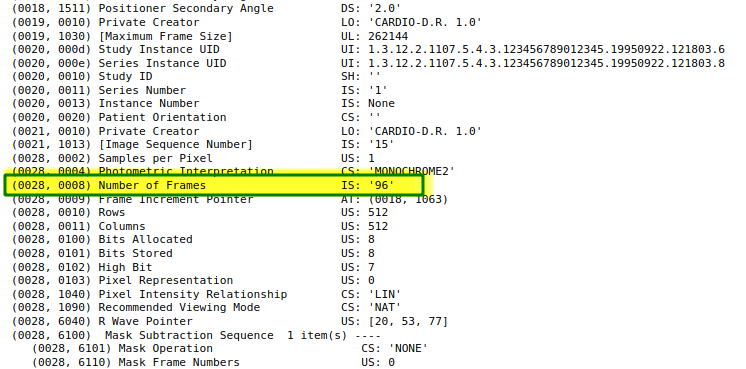
\includegraphics[width=9cm]{fig/number_of_frames.png}
    \legend{Fonte: Autor.}
    \label{fig:fig20}
\end{figure}

Para uma conversão em massa de uma base com muitas imagens é preciso tratar situações como esta, pois o processo de conversão, apesar de ser rápido para um único arquivo, pode demorar horas para grandes quantidades de imagens. Caso tais detalhes não sejam levados em consideração, um erro pode interromper a execução do programa de conversão e mais tempo terá de ser gasto para resolver o problema. O único arquivo \textit{DICOM} mostrado na imagem \ref{fig:fig20} possui 96 imagens e gerou todas as imagens mostradas na figura abaixo:

\begin{figure}[H]
    \centering
    \caption{Todas as imagens contidas no arquivo \textit{DICOM}.}
    \includegraphics[width=14cm]{fig/images_in_dicom.png}
    \legend{Fonte: Autor com imagens do \cite{cancer_imaging_archive_cancer_2022}.}
    \label{fig:fig21}
\end{figure}

Outro ponto do código contido na imagem \ref{fig:fig18} que deve ser explicado, são as linhas 11 e 12. Para salvar as imagens em um formato comum, é necessário converter seus pixeis para o valor correto. Por padrão as imagens contém pixeis com valores entre 0 e 255 e é isso que a linha 11 faz: normaliza os pixeis para um valor entre 0 e 255. E por fim, a linha 12 converte cada pixel para um inteiro de 8 bits.

Agora, a imagem está em um formato utilizável para treinar o modelo. Para fazer este procedimento em todas as imagens da base, o programa precisa ser alterado para ler os arquivos \textit{DICOM} do disco de forma automática e escrever os novos arquivos \textit{jpg} também de forma automatizada.

\subsection{Uniformização e redução da resolução}
\label{sec:uniformizacao}

Um dos requisitos necessários para se treinar o modelo é uma resolução uniforme em todas as imagens. Uniforme em alguns aspectos: largura e altura consistentes e ambas as dimensões devem ser múltiplas de \textbf{N}, onde \textbf{N} é a escala na qual o modelo será treinado para performar. \textbf{N} vale 4 para o contexto deste trabalho, já que o modelo treinado, será capaz de super resolver imagens em quatro vezes o tamanho original.

Não é necessário preocupar com a consistência entre largura e altura já que as imagens originalmente possuem altura e largura uniformes em todas as imagens selecionadas para treinamento. A segunda parte contudo, há de ser feita.

Transformar todas as milhares de imagens em imagens com resoluções múltiplas de 4 manualmente é uma tarefa completamente infactível. Alguma forma de automação deste processo é indispensável para a continuação do trabalho. Foi considerado o desenvolvimento de um software para tal, que fosse capaz de ler imagens do disco, encontrar sua resolução e redimensiona-la para o valor mais próximo que também fosse múltiplo de 4. O desenvolvimento e testes de tal ferramenta demandaria bastante tempo para ser implementado e testado. Se levada em consideração, a necessidade de que este software seja flexível à novas configurações (como novos valores para \textbf{N}, por exemplo), novas operações (como cortes em imagens, por exemplo), é razoável concluir com boa precisão, que ainda mais tempo seria desprendido para trabalhar na criação de uma ferramenta capaz de realizar todas estas tarefas.

Este desenvolvimento foi dispensado, pois um software de código aberto chamado \textit{Magick-Utils} não muito famoso, já faz a conversão da resolução de forma automatizada. Este software foi encontrado de forma inesperada, na descrição de um vídeo tutorial para o treinamento de uma implementação do modelo ESRGAN, e seu código é completamente aberto

\begin{figure}[H]
    \centering
    \caption{Captura de tela do software \textit{Magick-Utils}.}
    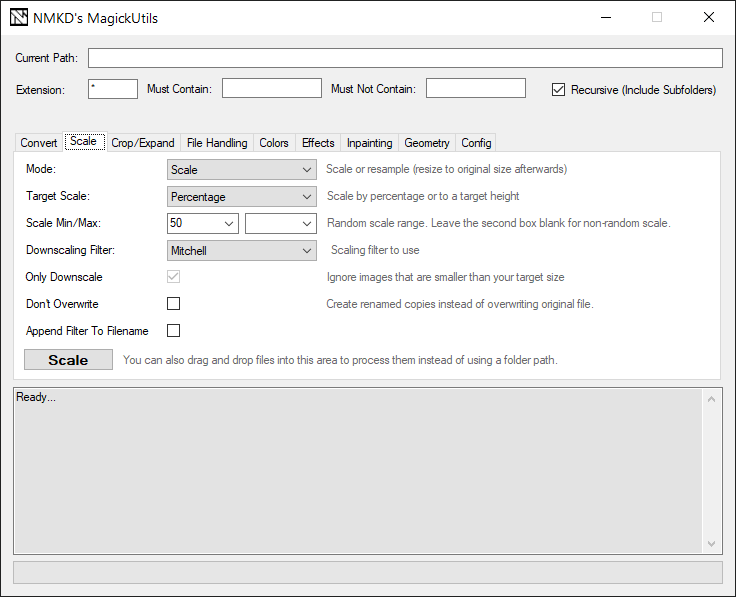
\includegraphics[width=14cm]{fig/magick-utils.png}
    \legend{Fonte: \textit{Github} do criador do software \cite{n00mkrad_magickutils_2022}. }
    \label{fig:fig22}
\end{figure}

O processo é relativamente lento, mas é possível fazer a conversão de todas as imagens em algumas horas.

Como descrito na seção \ref{sec:prep-imgs}, uma das formas de se controlar tempo e consumo de recursos do treinamento é reduzindo a resolução das imagens. Caso tal redução se faça necessária, o software \textit{Magick-Utils} \cite{n00mkrad_magickutils_2022} é perfeito para a tarefa. O programa suporta o usuário selecionar uma pasta inteira contendo dezenas de milhares de imagens. Este, irá alterar todas as imagens para uma resolução menor, até que as imagens estejam em um tamanho praticável para os recursos computacionais disponíveis para o treinamento.

\section{Considerações gerais sobre as imagens pós processadas}
\label{sec:desenvolvimento:general-considerations-post-processed-images}

Para sumarizar o estado das bases de imagens após o processamento descrito nas seções anteriores, segue a tabela abaixo:

\begin{table}[H]
    \centering
    \caption{Tabela sumarizando as imagens processadas.}
    \begin{tabular}{|l|l|l|} \hline
        \multirow{2}{*}{\textbf{Estatística}}   & \multicolumn{2}{|c|}{\textbf{Base de imagens}}            \\ \cline{2-3}
                                                & \textbf{Ressonância magnética}    & \textbf{Astronomia}   \\ \hline
        \textbf{Nº de imagens}                  & 6031                              & 243435                \\ \hline
        \textbf{Resolução}                      & 108x108                           & 424x424               \\ \hline            
        \textbf{Tamanho médio (bytes)}          & 4288.04                           & 12674.51              \\ \hline            
        \textbf{Tamanho 90º percentil (bytes)}  & 5314.6                            & 17674.51              \\ \hline            
        \textbf{Cor}                            & Monocromática (Tons de cinza)     & Colorida              \\ \hline            
    \end{tabular}
    \vspace{0.3cm}
    \legend{Fonte: Autor.}
    \label{tab:image_considerations}
\end{table}

Algumas das diferenças entres as bases de dados podem impactar no treinamento. A resolução das imagens astronômicas é quase quatro vezes maior que a resolução das imagens médica e em consequência, também medem mais de três vezes mais em disco.

Como se a diferença de resolução não bastasse, as imagens astronômicas são coloridas. A presença de cor aumenta, em algumas dimensões a estrutura de dados, neste caso, o tensor que irá trafegar nas redes. Enquanto uma imagem monocromática como as da base médica, pode ser representada com uma estrutura bidimensional. A imagem colorida requer mais uma dimensão para os canais de cores.

\begin{figure}[H]
    \centering
    \caption{Diagrama demonstrando diferença estrutural entre imagem monocromática e colorida.}
    \includegraphics[width=12cm]{fig/monochrome_vs_color.png}
    \legend{Fonte: Autor}
    \label{fig:monochrome_vs_color}
\end{figure}

Na figura \ref{fig:monochrome_vs_color}, a imagem A representa uma imagem monocromática, com apenas duas dimensões: altura e largura. A imagem B, representa uma imagem colorida com cores RGB. Uma dimensão a mais é necessária para armazenamento e processamento: os canais de cores.

\section{Preparação do ambiente para treinamento}
\index{Treinamento}
\label{sec:environment-prep-training}


Nesta parte do trabalho, é descrita toda a configuração, e tentativas de configuração, necessárias para o treinamento correto do modelo ESRGAN. Detalhes do hardware disponível e utilizado são apresentados, assim como também especificações de software como sistema operacional, bibliotecas utilizadas, forma de executar o treinamento etc.

O modelo utilizado, consiste em uma implementação de terceiros da especificação da ESRGAN já que entender os pormenores deste modelo é um esforço muito além do escopo do trabalho. Como utilizar tal software, envolve lidar com softwares e implementações externos, é preciso ater-se aos detalhes disponibilizados para que seja possível configurar o ambiente e preparar as entradas de forma correta.

Antes da descrição mais acurada do processo, é fundamental deixar claro os requisitos necessários para utilizar uma ESRGAN. O modelo, como explicado anteriormente consiste de várias camadas de processamento. Cada uma destas, executa uma quantidade significativa de cálculos cada vez que o modelo é alimentado com dados de entrada, seja em fase de treinamento, testes ou na utilização real.

Modelos como este, assim como diversos outros tipos de modelos de inteligência artificial, conseguem tirar bastante proveito de processadores com vários núcleos. Estes processadores conseguem, quando implementado de tal forma, realizar uma grande quantidade de cálculos simultaneamente. Cálculos que individualmente são simples operações matemáticas, mas quando combinados da forma correta, representam todo o modelo que este trabalho analisa. Um tipo de processador que se encaixa nesta categoria, são as GPUs (Graphics Processing Unit, unidade de processamento de gráficos, do inglês).\index{GPU} Vários dispositivos domésticos vêm de fábrica com uma GPU dedicada que possui centenas, senão milhares de núcleos.

Com isso em mente, diversos modelos e bibliotecas de computação numérica e inteligência artificial são desenvolvidos com a ideia de que serão treinadas, testadas e utilizadas em GPUs, em mente. Vários testes de performance demonstram a superioridade das GPUs em comparação com os processadores tradicionais (CPUs)\index{CPU} para tarefas de treinamento de modelos de inteligência artificial. De acordo com \citeonline{pantigoso_velasquez_performance_2019}, para modelos mais complexos é notável a diferença de desempenho quando se utiliza de GPUs para o treinamento. Esta diferença no entanto, decresce com modelos mais simples.

Para usufruir deste hardware, é necessário no entanto de uma forma de interface para que o modelo, implementado utilizando uma tecnologia \textbf{X}, representando qualquer variação do modelo feito com tecnologias distintas, possa acessar os recursos da GPU, independente do modelo. É esse o papel do CUDA. Uma ferramenta desenvolvida pela \textit{NVIDIA} para fazer esse interfaceamento. CUDA, de acordo com a própria empresa por trás da ferramenta, é uma plataforma de computação paralela que engloba diversos recursos. A ferramenta é capaz de compilar código para executar em GPUs, usar interfaces em diferentes linguagens para acessar recursos do hardware entre outras coisas. Os desenvolvedores que utilizam CUDA, determinam quais partes do código devem ser executadas de forma paralela e demarcam este trecho com anotações. O compilador ou interpretador então, detecta estes trechos e os executa em núcleos paralelos na GPU.

Várias destas bibliotecas utilizadas para desenvolver modelos de inteligência artificial e redes neurais fazem uso de recursos matemáticos como tensores, que generalizam várias estruturas básicas: valores escalares, vetores, matrizes etc. Existem hardwares específicos para processamento de tensores, os assim chamados TPUs (Tensor Processing Unit, unidade de processamento de tensores, do inglês) e inclusive, há formas de acessá-los de forma gratuita. Como o modelo utilizado neste trabalho foi desenvolvido e otimizado para GPUs, é supérfluo entrar em mais detalhes sobre TPUs. Vale no entanto, a menção e talvez um trabalho futuro envolvendo o assunto.\index{TPU}

\subsection{Descrevendo o hardware disponível}
\index{Treinamento}

Para treinar o modelo, um computador esteve disponível. A especificação de seu hardware está contida na tabela abaixo:

\begin{table}[H]
    \centering
    \caption{Tabela de descrição do hardware}
    \begin{tabular}{|l|l|} \hline
        \textbf{Item}            & \textbf{Descrição}                    \\ \hline
        CPU                      & Intel i7 Octa Core                    \\ \hline
        Memória RAM              & 16GB                                  \\ \hline
        Memória de Vídeo         & 2GB                                   \\ \hline
        Modelo da placa de vídeo & GeForce MX350                         \\ \hline
        Disco                    & 512GB (apenas 90GB disponível)        \\ \hline
        Sistema operacional      & Windows 10 e Ubuntu 24.04 disponível  \\ \hline
    \end{tabular}
    \vspace{0.3cm}
    \legend{Fonte: Autor.}
    \label{tab:my_label}
\end{table}

A placa de vídeo apresentada (GeForce GT920M) é um modelo de computadores portáteis voltada para jogos. Uma informação importante de se documentar, é sua quantidade de Núcleos \textit{CUDA}\index{CUDA} conhecidos popularmente pelo termo em inglês \textit{Cuda Core}. Os núcleos \textit{CUDA} são os núcleos de processamento de instruções das \textit{GPUs} da \textit{NVIDIA}, conceito bem parecido com o conceito de núcleos de processadores \cite{ryles_what_2022}. A placa em questão possui compatibilidade com \textit{CUDA}, um requisito indispensável, e possui 384 núcleos \textit{CUDA} \cite{nvidia_geforce_2022, technical_city_nvidia_2022}. Esta placa de vídeo de entrada possui 96 vezes mais núcleos que a CPU disponível.

O hardware descrito, está distante de ser o ideal para o treinamento de um modelo complexo e exigente em termos de recursos, como é o caso do modelo descrito e utilizado neste trabalho. Treinamentos do tipo costumam ser feitos em servidores dedicados, com processadores poderosos e grandes quantidades de memória RAM e memória de vídeo (VRAM).

Por causa desta limitação de recursos, é preciso recorrer à alternativas a nível de software, como descrito na seção \ref{sec:prep-imgs}.


\subsection{Descrição do software necessário para treinar o modelo}

Para treinar, executar e utilizar o modelo de forma geral, as dependências da implementação utilizada devem ser satisfeitas. Ou seja, é preciso antes, instalar as bibliotecas, \textit{frameworks} etc. necessários para a execução do modelo.

Nesta seção será descrito, com o maior nível de detalhes possível, como este processo é realizado. Da preparação do ambiente até à execução do treinamento e do modelo em si. Tenha em mente que esta etapa, apesar de parecer simples (afinal, consiste apenas em instalar softwares e no máximo fazer uma eventual configuração), pode ser bastante complicada por alguns motivos.

O primeiro passo nesta tarefa é reproduzir o ambiente onde o modelo foi desenvolvido e testado. Reproduzir um ambiente qualquer, requer manter todas as bibliotecas e softwares em geral, na mesma versão que o ambiente desejado, ou pelo menos manter tudo em uma versão compatível. Caso o(s) desenvolvedor(es) do modelo forneçam estas informações, grande parte do esforço está adiantado. Caso estas informações não estejam disponíveis, estas precisam, de forma não negociável, ser encontradas, seja buscando em fóruns ou outras fontes elaboradas por pessoas que passaram pelo mesmo problema, ou por tentativa e erro.

O segundo motivo complicador desta fase do trabalho, é a compatibilidade entre software e hardware. Como explicado anteriormente, reproduzir o ambiente a nível de software requer encontrar uma interseção de compatibilidade entre todas as dependências necessárias para executar o modelo. O mesmo acontece com hardware. Alguns dispositivos, como \textit{GPUs}, que são extremamente necessárias para este trabalho, possuem \textit{drivers} específicos em versões específicas, que integram com versões particulares de bibliotecas necessárias. Até aí, nenhuma novidade em relação aos problemas de software. Quando tratamos de hardware no entanto, não se pode contar com versões atualizadas de determinado \textit{driver} para sempre. Os desenvolvedores podem interromper o suporte de uma \textit{GPU} A, mais antiga e obsoleta, para concentrarem os esforços num modelo B, mais atualizado. Isto pode ser um problema comprometedor, especialmente quando há uma limitação tão grande de hardware como é o caso deste trabalho.

\subsubsection{Experimentos preliminares com o ambiente}

Os primeiros experimentos de preparação do ambiente foram feitos em um computador com uma instalação do sistema operacional Ubuntu versão 18.04LTS. Várias fontes informais como vídeos e comentários em fóruns e redes sociais sobre o assunto recomendaram o uso de uma distribuição Linux qualquer para o treinamento de modelos complexos e pesados como o modelo atual. As recomendações sempre levavam em consideração a forma como os sistemas operacionais Linux gerenciam os recursos de forma mais minimalista, deixando mais memória, processador e disco disponíveis para o treinamento em si. Além disso, Linux pareceu uma boa primeira alternativa, devido à familiaridade de uso.

Contudo, os experimentos no Linux foram um insucesso. Como parte das dependências são fornecidas pela empresa \textit{NVIDIA}, suas bibliotecas proprietárias precisam ser instaladas no Linux e isso nem sempre é uma tarefa simples. No experimento realizado, ao instalar o \textit{driver} necessário para utilizar a \textit{GPU}, várias funcionalidades básicas do sistema operacional pararam de funcionar propriamente.

Como uma instalação do Windows 10 estava disponível, não valeria o esforço de tentar resolver os diversos problemas de compatibilidade entre dependências da \textit{NVIDIA} e o sistema operacional, o desenvolvimento prosseguiu utilizando como sistema operacional, o Windows 10.

\subsubsection{Breve descrição sobre versões}
\label{sec:environment-version-compatability}

Para fazer qualquer procedimento com este modelo, seja treinamento, teste ou execução, vários níveis de compatibilidade de software com software e de software com hardware precisam ser garantidos. O diagrama abaixo ilustra a interação entre as partes:

\begin{figure}[H]
    \centering
    \caption{Diagrama de interação entre as partes envolvidas no modelo.}
    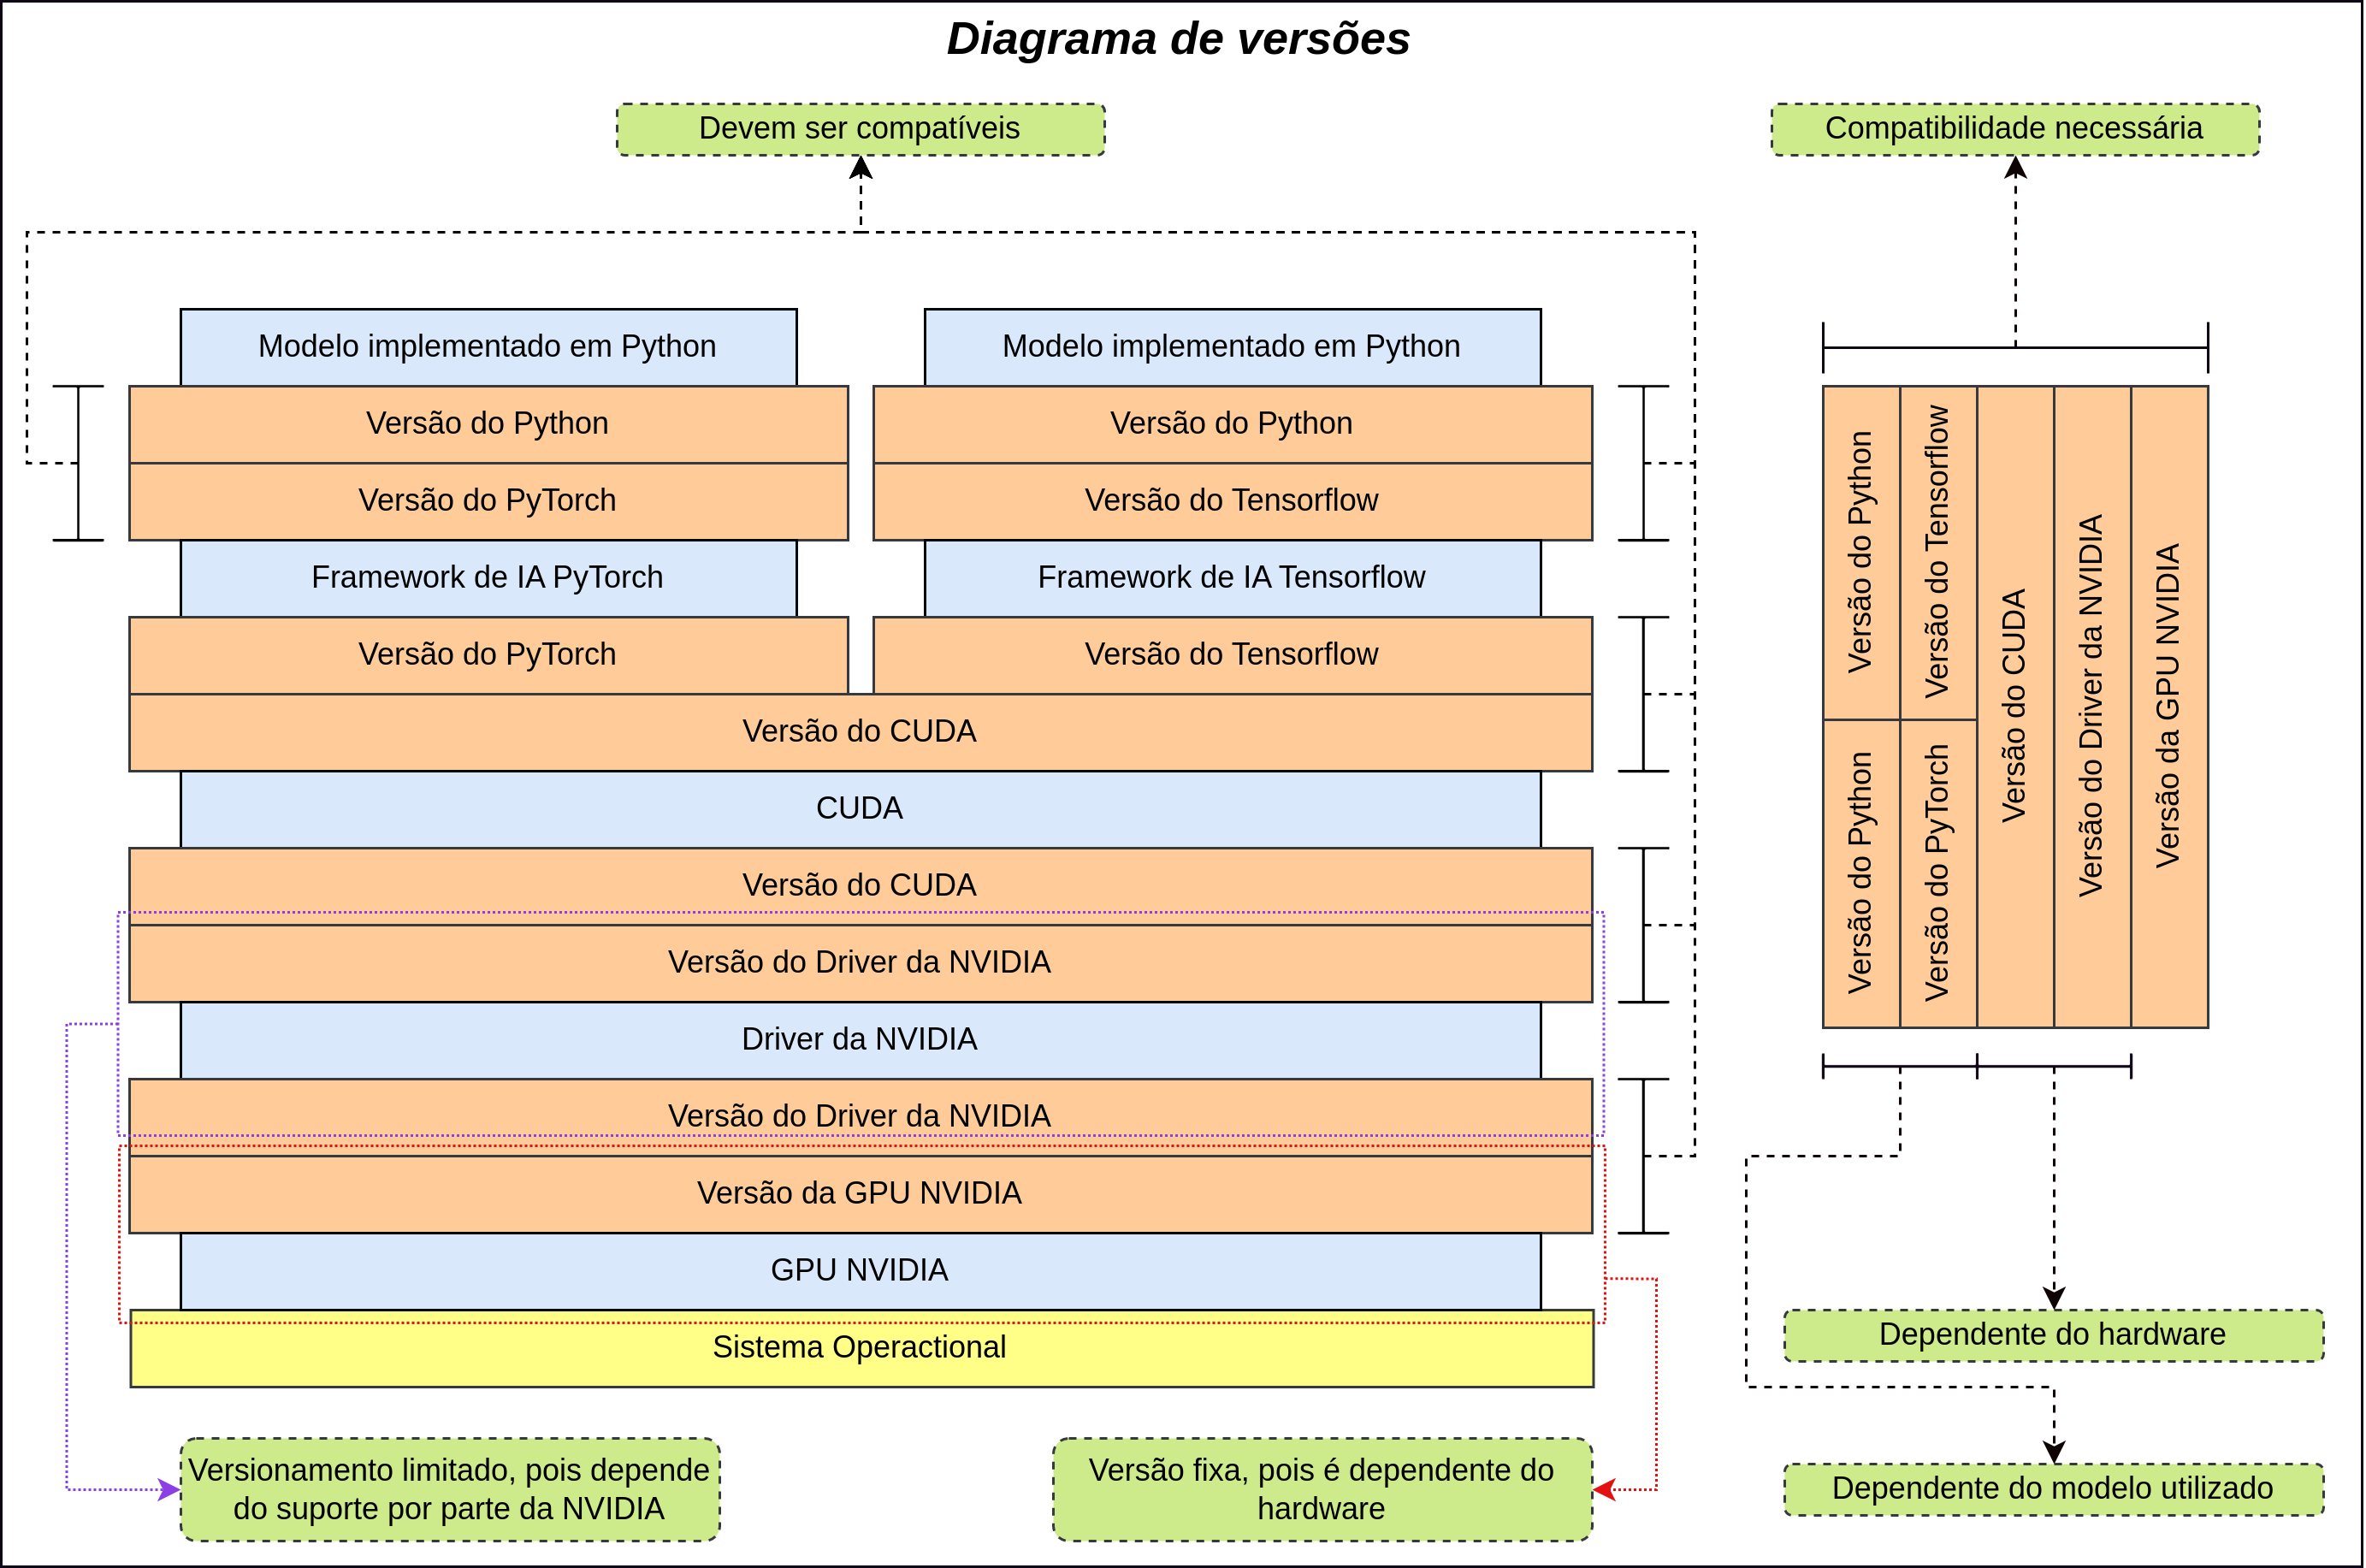
\includegraphics[width=14cm]{fig/version_diagram.png}
    \legend{Fonte: Autor.}
    \label{fig:fig24}
\end{figure}

Na figura \ref{fig:fig24}, os blocos laranja fazendo contato entre si representam compatibilidade de comunicação entre as partes. Ao todo são quatro níveis de compatibilidade. As versões do \textit{python} e dos frameworks (\textit{PyTorch} e \textit{Tensorflow}) já são predeterminadas pela implementação do modelo. A dificuldade vem em encontrar uma versão do CUDA que se comunica com a versão dos frameworks e do \textit{driver} e uma versão do \textit{driver} que se comunica com o hardware em si.

\subsubsection{Instalação do \textit{driver} da \textit{NVIDIA}}
\label{sec:driver}
\index{NVIDIA}
\index{GPU}

O passo base para prosseguir com a instalação das dependências, é instalar um \textit{driver} compatível com ambos, a placa de vídeo disponível, e a versão das bibliotecas utilizadas.

Esta seção, apesar de ter sido colocada imediatamente anterior à seção sobre \textit{CUDA}\index{CUDA} (vide seção \ref{sec:cuda}) devido à ordem cronológica correta e esperada dos passos, foi desenvolvida em repetição antes e após a instalação do \textit{CUDA}. Isto aconteceu por inúmeros problemas de compatibilidade que apareceram ao tentar integrar o \textit{driver} com a biblioteca e estes dois com o hardware em si. O processo é extremamente demorado e mecânico. Como a instalação e desinstalação tomam bastante tempo por si só, é de se esperar que fazê-los várias vezes até obtermos uma combinação compatível entre si, tomaria muito tempo.

Para encontrar o \textit{driver} específico ao \textit{hardware} (GPU) disponível, basta buscar no mecanismo oficial de busca de \textit{drivers} atualizados do site da \textit{NVIDIA} (figura \ref{fig:fig23}).

\begin{figure}[H]
    \centering
    \caption{Captura de tela do buscador de drivers da \textit{NVIDIA}.}
    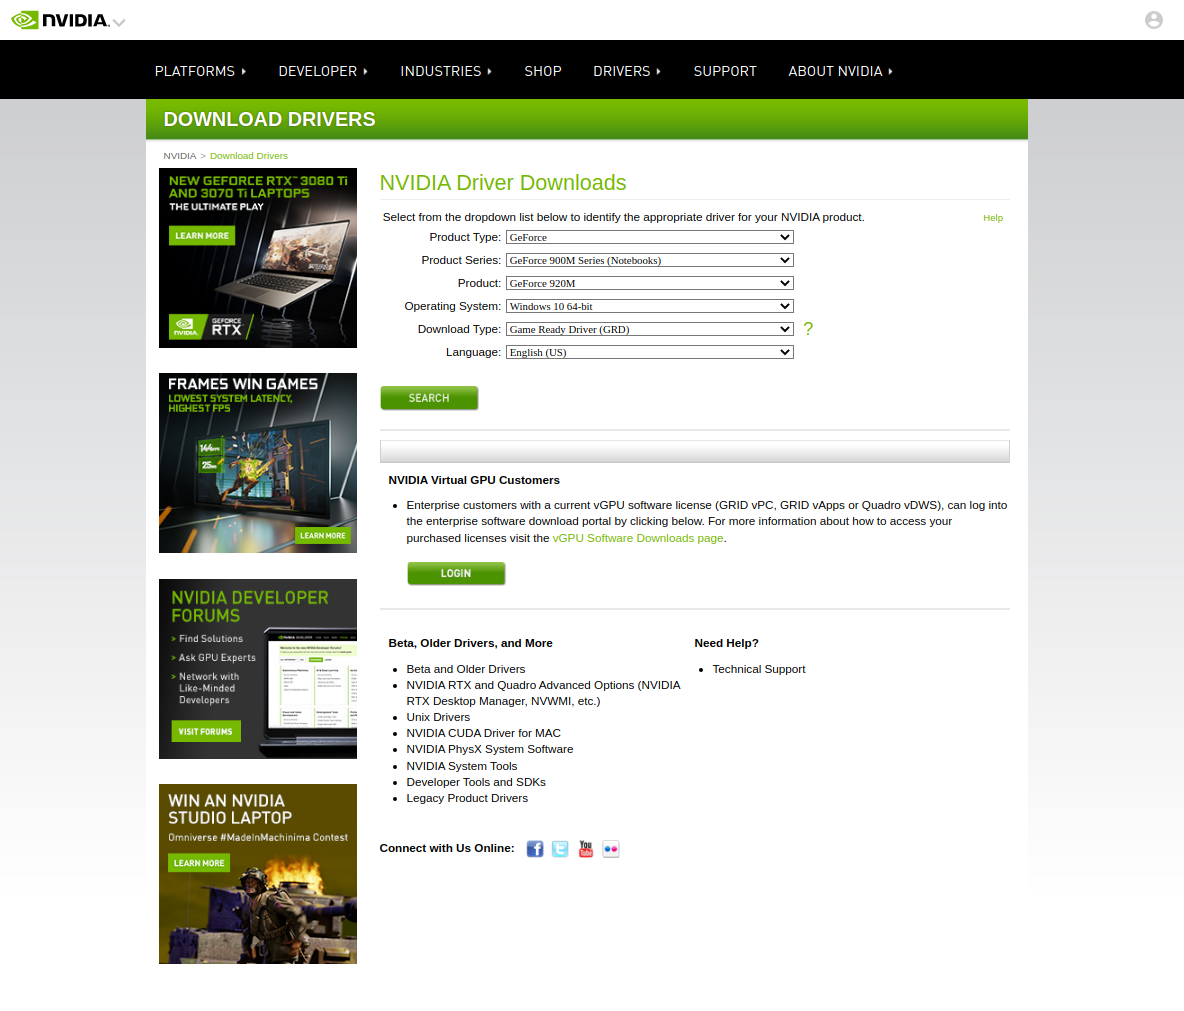
\includegraphics[width=14cm]{fig/nvidia_driver.png}
    \legend{Fonte: Buscador de \textit{drivers} atualizados da \textit{NVIDIA} \cite{nvidia_download_2023} }
    \label{fig:fig23}
\end{figure}

Caso, por motivos de compatibilidade o \textit{driver} atualizado não integre com as bibliotecas necessárias para o desenvolvimento, existe ainda a alternativa de procurar por versões anteriores ou versões de teste do \textit{driver} para o hardware. A figura \ref{fig:fig24} mostra o buscador avançado de \textit{drivers} que a \textit{NVIDIA} disponibiliza. Nele, dispõe-se várias opções com as quais é possível experimentar. Basta buscar pelo modelo do seu hardware, filtrando pelas várias opções disponíveis.

\begin{figure}[H]
    \centering
    \caption{Captura de tela do buscador avançado de drivers da \textit{NVIDIA}.}
    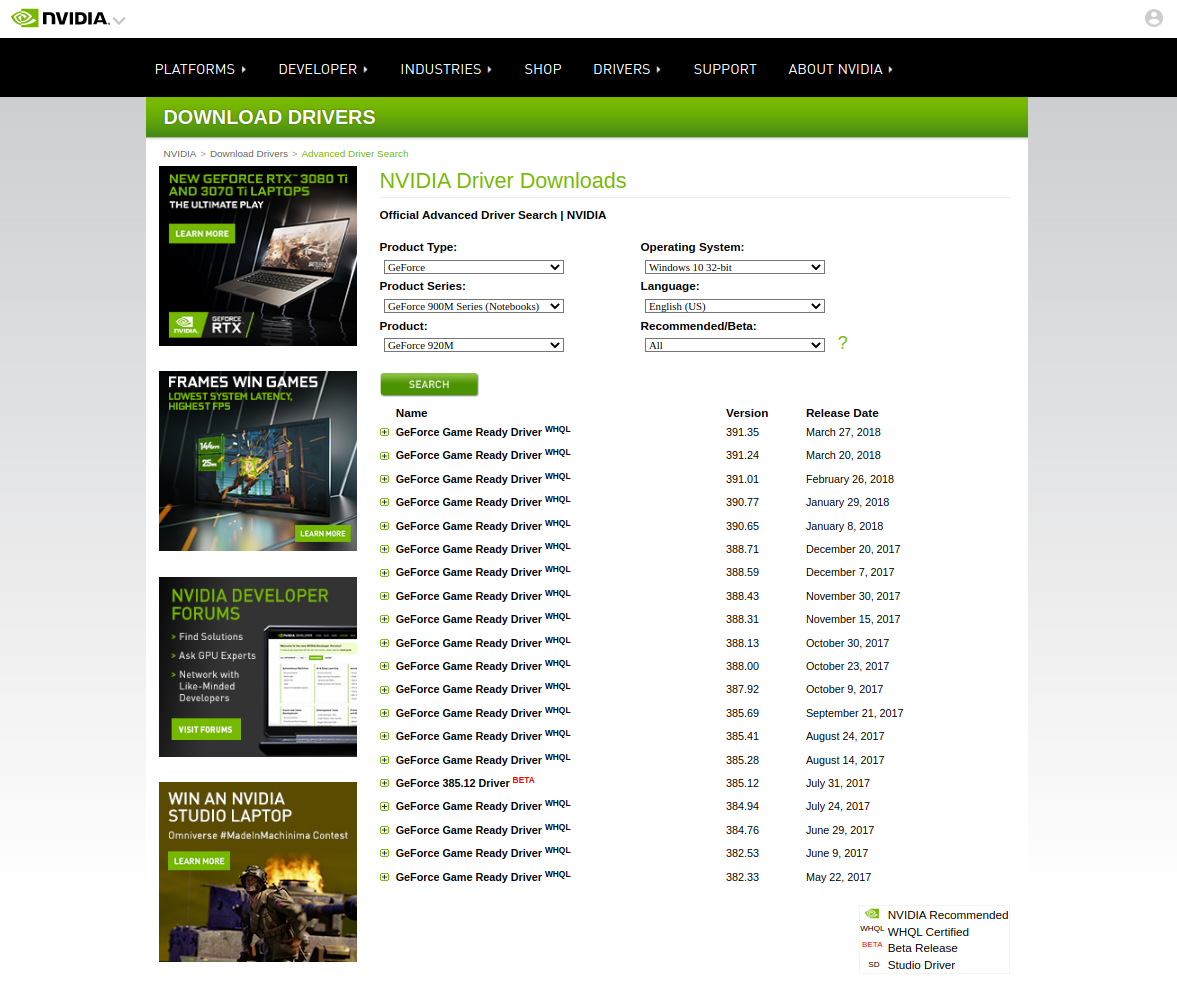
\includegraphics[width=14cm]{fig/nvidia_driver_advanced.png}
    \legend{Fonte: Buscador avançado de \textit{drivers} da \textit{NVIDIA} \cite{nvidia_advanced_2023} }
    \label{fig:nvidia-site:fig24}
\end{figure}

Após encontrar o \textit{driver} específico, basta fazer o \textit{download}, executar o arquivo e seguir os passos para instalação. A instalação contém várias opções e componentes mais voltadas para cenários específicos. As opções padrão geralmente são suficientes para a maior parte dos casos, de acordo com os testes realizados. Além da instalação do \textit{driver}, algumas atualizações podem ser necessárias. O instalador é capaz de resolvê-las por conta própria.

\subsubsection{Instalação do CUDA}
\label{sec:cuda}
\index{CUDA}
\index{NVIDIA}

Esta parte precisa de ser realizada em perfeita harmonia com a seção \ref{sec:driver}. Qualquer versão incorreta pode impedir o funcionamento do projeto como um todo.

A primeira parte da instalação, como esperado, é baixar o instalador. Isso pode ser feito através do site da \textit{NVIDIA Developers}. Um site voltado para usuários mais técnicos que desenvolvem para as plataformas da \textit{NVIDIA}.

\begin{figure}[H]
    \centering
    \caption{Captura de tela do site da \textit{NVIDIA Developers}.}
    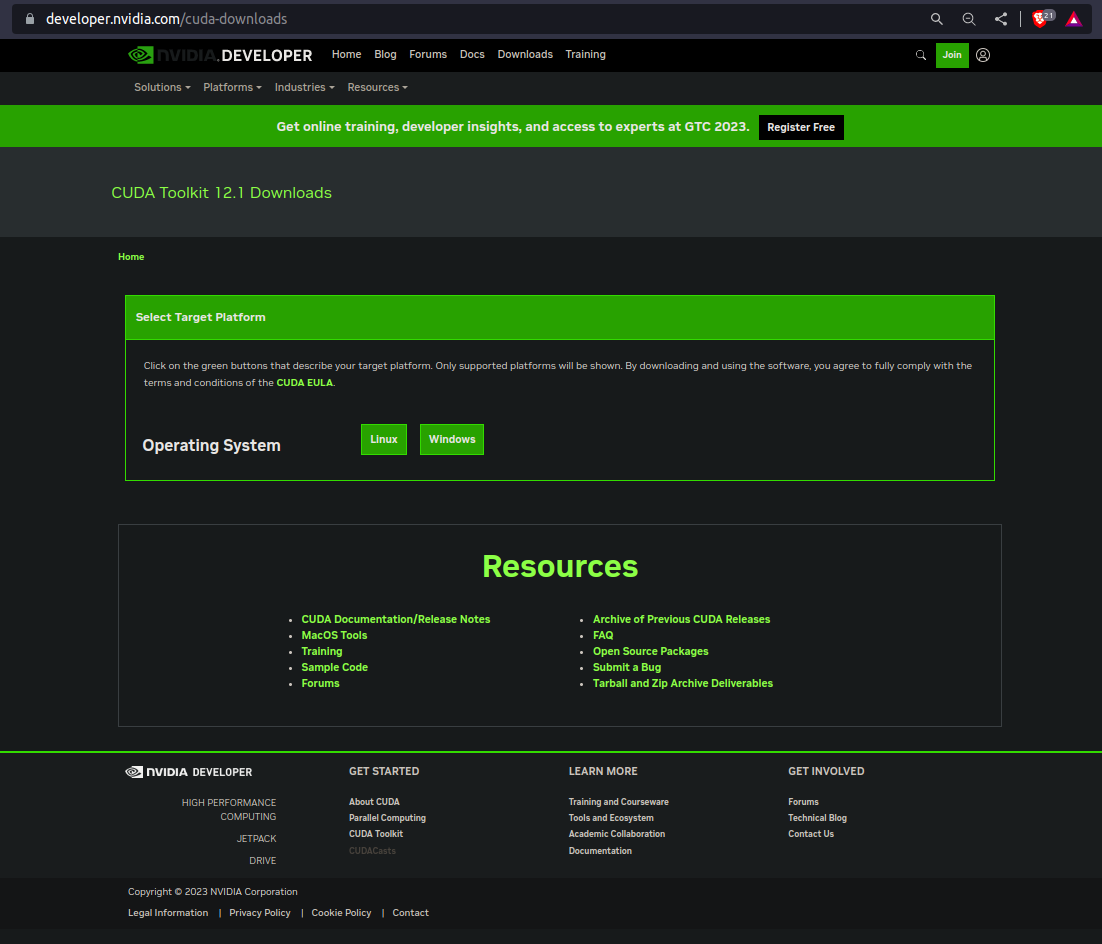
\includegraphics[width=12cm]{fig/cuda_download_page.png}
    \legend{Fonte: Buscador de instaladores CUDA \cite{nvidia_cuda_2024}. }
    \label{fig:fig25}
\end{figure}

A figura \ref{fig:fig25} mostra a página inicial do site. Para encontrar o instalador correto para cada situação, preencha o filtro com os detalhes desejados.

\begin{figure}[H]
    \centering
    \caption{Captura de tela do filtro do buscador de instaladores CUDA.}
    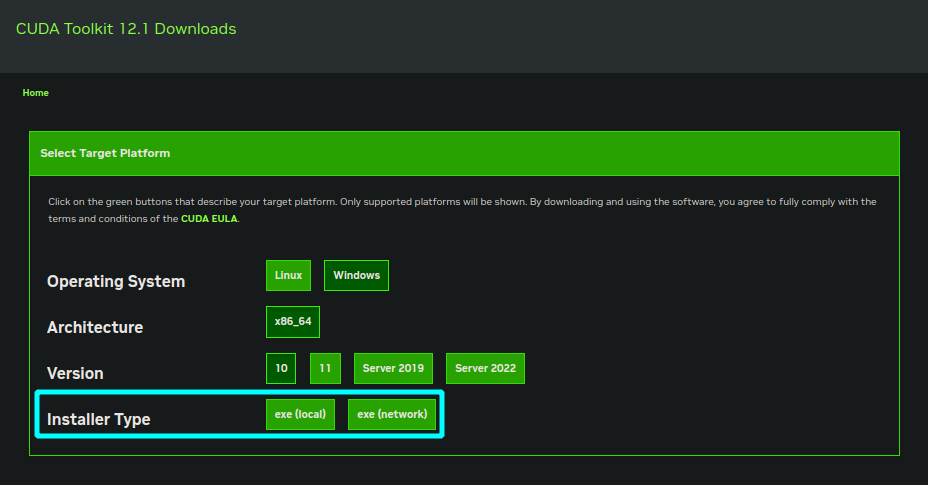
\includegraphics[width=12cm]{fig/cuda_download_page_installer_type.png}
    \legend{Fonte: Filtros do buscador de instaladores CUDA \cite{nvidia_cuda_2024}. }
    \label{fig:fig26}
\end{figure}

Com os filtros da figura \ref{fig:fig26} preenchidos, serão disponibilizadas duas versões para download (\textit{Installer type}, tipo do instalador, do inglês): o instalador completo (opção \textit{local}) e o instalador pela rede (opção \textit{network}). O instalador completo faz um download lento e grande mas uma vez baixado, nenhum download extra será necessário. O segundo, pela rede, baixa um instalador mais compacto e, durante a instalação faz o download do restante. Ambas opções trarão o mesmo resultado. Após a escolha do tipo de instalador, um botão para o download será exibido.

\begin{figure}[H]
    \centering
    \caption{Captura de tela da busca de instaladores CUDA.}
    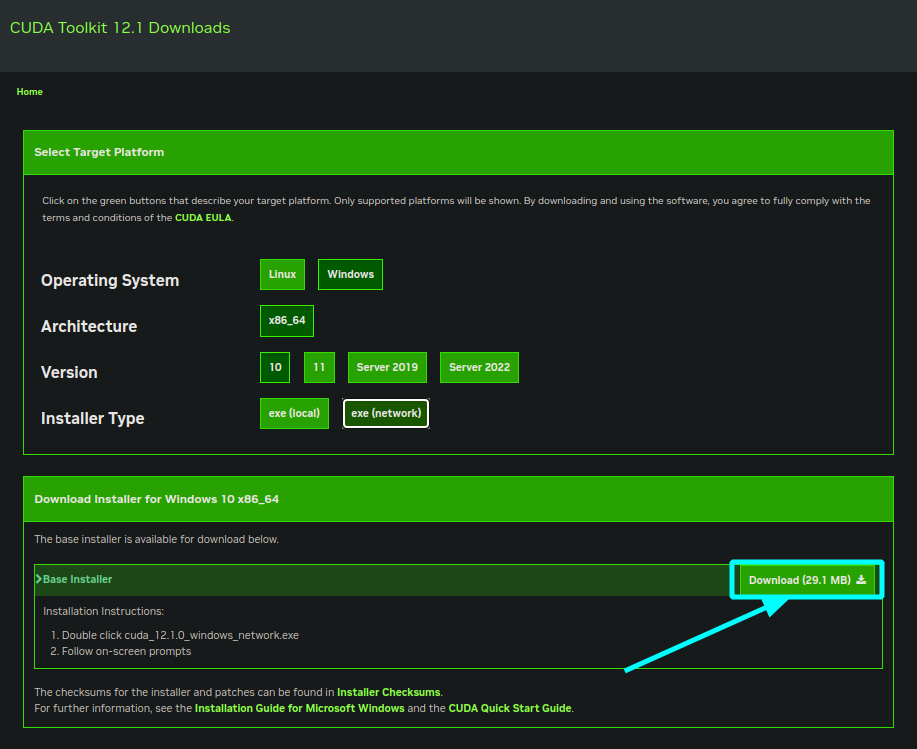
\includegraphics[width=10cm]{fig/cuda_download_page_final.png}
    \legend{Fonte: Busca completa de instaladores CUDA \cite{nvidia_cuda_2024}. }
    \label{fig:fig27}
\end{figure}

Faça o download, clicando no botão destacado na figura \ref{fig:fig27} e execute o arquivo baixado.

\index{CUDA}
\begin{figure}[H]
    \centering
    \caption{Captura de tela de instalação CUDA.}
    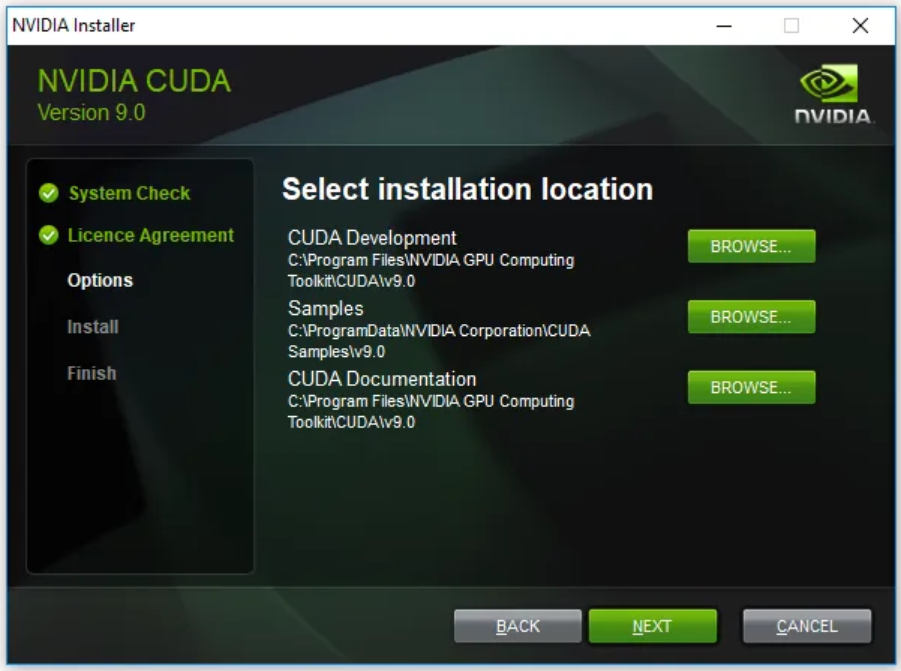
\includegraphics[width=10cm]{fig/cuda_instalacao.png}
    \legend{Fonte: Tela do instalador CUDA. \cite{kitson_installing_2022}}
    \label{fig:fig28}
\end{figure}

Nas opções do instalador acima, serão disponibilizadas a versão expressa e a versão avançada. A versão expressa, de instalação mais rápida, é suficiente para o propósito desta instalação. Siga os passos normalmente até finalizar. Esta instalação pode tomar um tempo considerável, dependendo do tipo de instalador escolhido. Caso a opção rede (\textit{network}) tenha sido a escolhida, a maior parte do software será baixada durante a instalação, justificando assim a demora extra.

\subsection{Apresentação do modelo}

Nesta subseção, detalhes sobre a implementação do modelo, assim como características de configurações serão descritos.

\subsubsection{Descrevendo a implementação}

Algumas implementações foram utilizadas durante os experimentos. Cada uma delas, fornece uma abordagem diferente para a mesma arquitetura, apesar de compartilharem o mesmo objetivo final. Uma das principais diferenças encontradas entre implementações distintas, são as ferramentas utilizadas para desenvolvê-las. Sejam versões diferentes ou ferramentas completamente diferentes.

O requisito necessário para que uma destas implementações sejam adequadas para o trabalho é interoperabilidade com os drivers e hardwares disponíveis. No final das contas, as implementações utilizadas podem ser divididas em dois grupos:

\begin{itemize}
    \item Modelos implementados utilizando a biblioteca \textit{Tensorflow}
    \item Modelos implementados utilizando a biblioteca \textit{PyTorch}
\end{itemize}

Ambas as bibliotecas são extremamente populares no meio científico de aprendizado de máquinas e computação numérica em geral. Estas bibliotecas abstraem parte da complexidade matemática por trás das construções e execuções dos modelos, dando à pessoa que está desenvolvendo, uma linguagem mais declarativa e de alto nível para expressar suas intenções. Toda a parte algébrica por trás do modelo, é então trabalhada pela biblioteca. Otimizações e transformações são feitas, para maximizar o aproveito do hardware, livrando assim, o(a) desenvolvedor(a) final de tais aperfeiçoamentos.

Após várias tentativas com modelos baseados no Tensorflow, foi concluído que, dado o recurso computacional disponível, estes modelos não iriam trazer resultados satisfatórios em tempo hábil. Os treinamentos com os modelos em Tensorflow testados, produziam erros de memória insuficiente para treinamento, horas após o início do processo.

Treinar as redes só foi possível com os modelos em Tensorflow utilizados, quando os parâmetros de treinamentos eram absurdamente baixos (e.g. uma imagem carregada por vez, i.e. um \textit{batch\_size} de 1). Isso por si só iria deteriorar consideravelmente a qualidade dos resultados, dentro do tempo disponível para treinamento que inicialmente, compreendia o período noturno, quando a máquina não estava sendo utilizada. Ou seja, os modelos baseados no Tensorflow iriam tomar um tempo impraticável para atingir um número \textbf{n} de épocas.

Além disso, nem todos os modelos em Tensorflow eram executáveis na máquina utilizada, seja por incompatibilidade de versões das bibliotecas, seja por erros de configuração. 

No final das contas, um modelo baseado em PyTorch foi o escolhido. Este modelo possui certa complexidade para se configurar, mas diferente dos modelos em Tensorflow testados anteriormente, as falhas acontecem cedo, permitindo assim melhor adaptabilidade no treinamento. O consumo de memória deste modelo, também foi significativamente menor, com parâmetros pequenos (mas não tão pequenos a ponto de delongar muito o treinamento), é possível utilizar a máquina para outras tarefas paralelas, algo infactível nos modelos anteriores. 

O modelo de código aberto \textit{BasicSR} \cite{blueamulet_blueamuletbasicsr_2023}, foi o modelo eleito. O projeto em si, contém outras implementações e capacidades, mas para o escopo desse trabalho, o foco principal foi sob o módulo de ESRGAN com super resolução de quatro vezes das imagens de entrada. A implementação é baseada no modelo de ESRGAN anteriormente citado neste trabalho \cite{wang_esrgan_2018}.


\subsubsection{Detalhando a preparação do projeto para treinamento}
\label{sec:preping-project-for-training}

Para executar a implementação, seja treinamento ou execução, esta antes, deve ser configurada. O projeto utilizado requer duas configurações básicas além obviamente, das dependências descritas anteriormente (driver da NVIDIA e CUDA). Primeiramente um modelo pré-treinado inicial deve ser encontrado assim como um arquivo de configurações contendo os dados que o modelo precisa para funcionar propriamente, como caminho para o diretório com os dados de treinamento, qual algoritmo de treinamento utilizar, etc.

Os modelos pré-treinados podem ser encontrados juntos com o projeto da implementação do modelo. Uma característica muito importante que deve ser levada em consideração é a arquitetura do modelo pré-treinado. Essa arquitetura deve ser idêntica à arquitetura para a qual o modelo irá ser treinado, ou seja, se uma ESRGAN para fazer super resolução de quatro vezes será treinada, obrigatoriamente, um modelo pré-treinado de ESRGAN com super resolução de quatro vezes deve ser utilizado. Qualquer outra variação não irá funcionar, devido à falta de compatibilidade da estrutura interna das camadas e pesos entre uma arquitetura e outra.

Após obtido o modelo pré-treinado, deve se organizar os dados de treinamento de uma maneira específica para que a implementação possa entender e configurar o projeto. Como o objetivo é obter um modelo treinado capaz de super resolver imagens em quatro vezes sua resolução inicial, as bases de dados devem estar dispostas com as seguintes características:

\begin{enumerate}
    \item Uma base de dados de treinamento, contendo:
    \begin{itemize}
        \item Imagens em baixa resolução 
        \item A versão de alta resolução (quatro vezes a resolução) das imagens de baixa resolução
    \end{itemize}
    \item Uma base de dados de validação, contendo:
    \begin{itemize}
        \item Imagens em baixa resolução
        \item A versão de alta resolução (quatro vezes a resolução) das imagens de baixa resolução
    \end{itemize}
\end{enumerate}

A proporção de dados separados para cada uma das duas bases de dados foi de 80:20: 80\% das imagens dedicadas à treinamento, e 20\%, dedicadas à validação. Para gerar as imagens de baixa resolução, a partir das imagens de alta resolução, o processo descrito na seção \ref{sec:uniformizacao} foi utilizado. 

Com as imagens preparadas e distribuídas em diretórios específicos, de acordo com a descrição anterior, os caminhos onde cada uma das divisões da base de dados se encontra podem ser adicionados no arquivo de configuração do projeto.

\begin{figure}[H]
    \centering
    \caption{Trecho do arquivo de configuração para treinamento e execução da implementação do modelo.}
    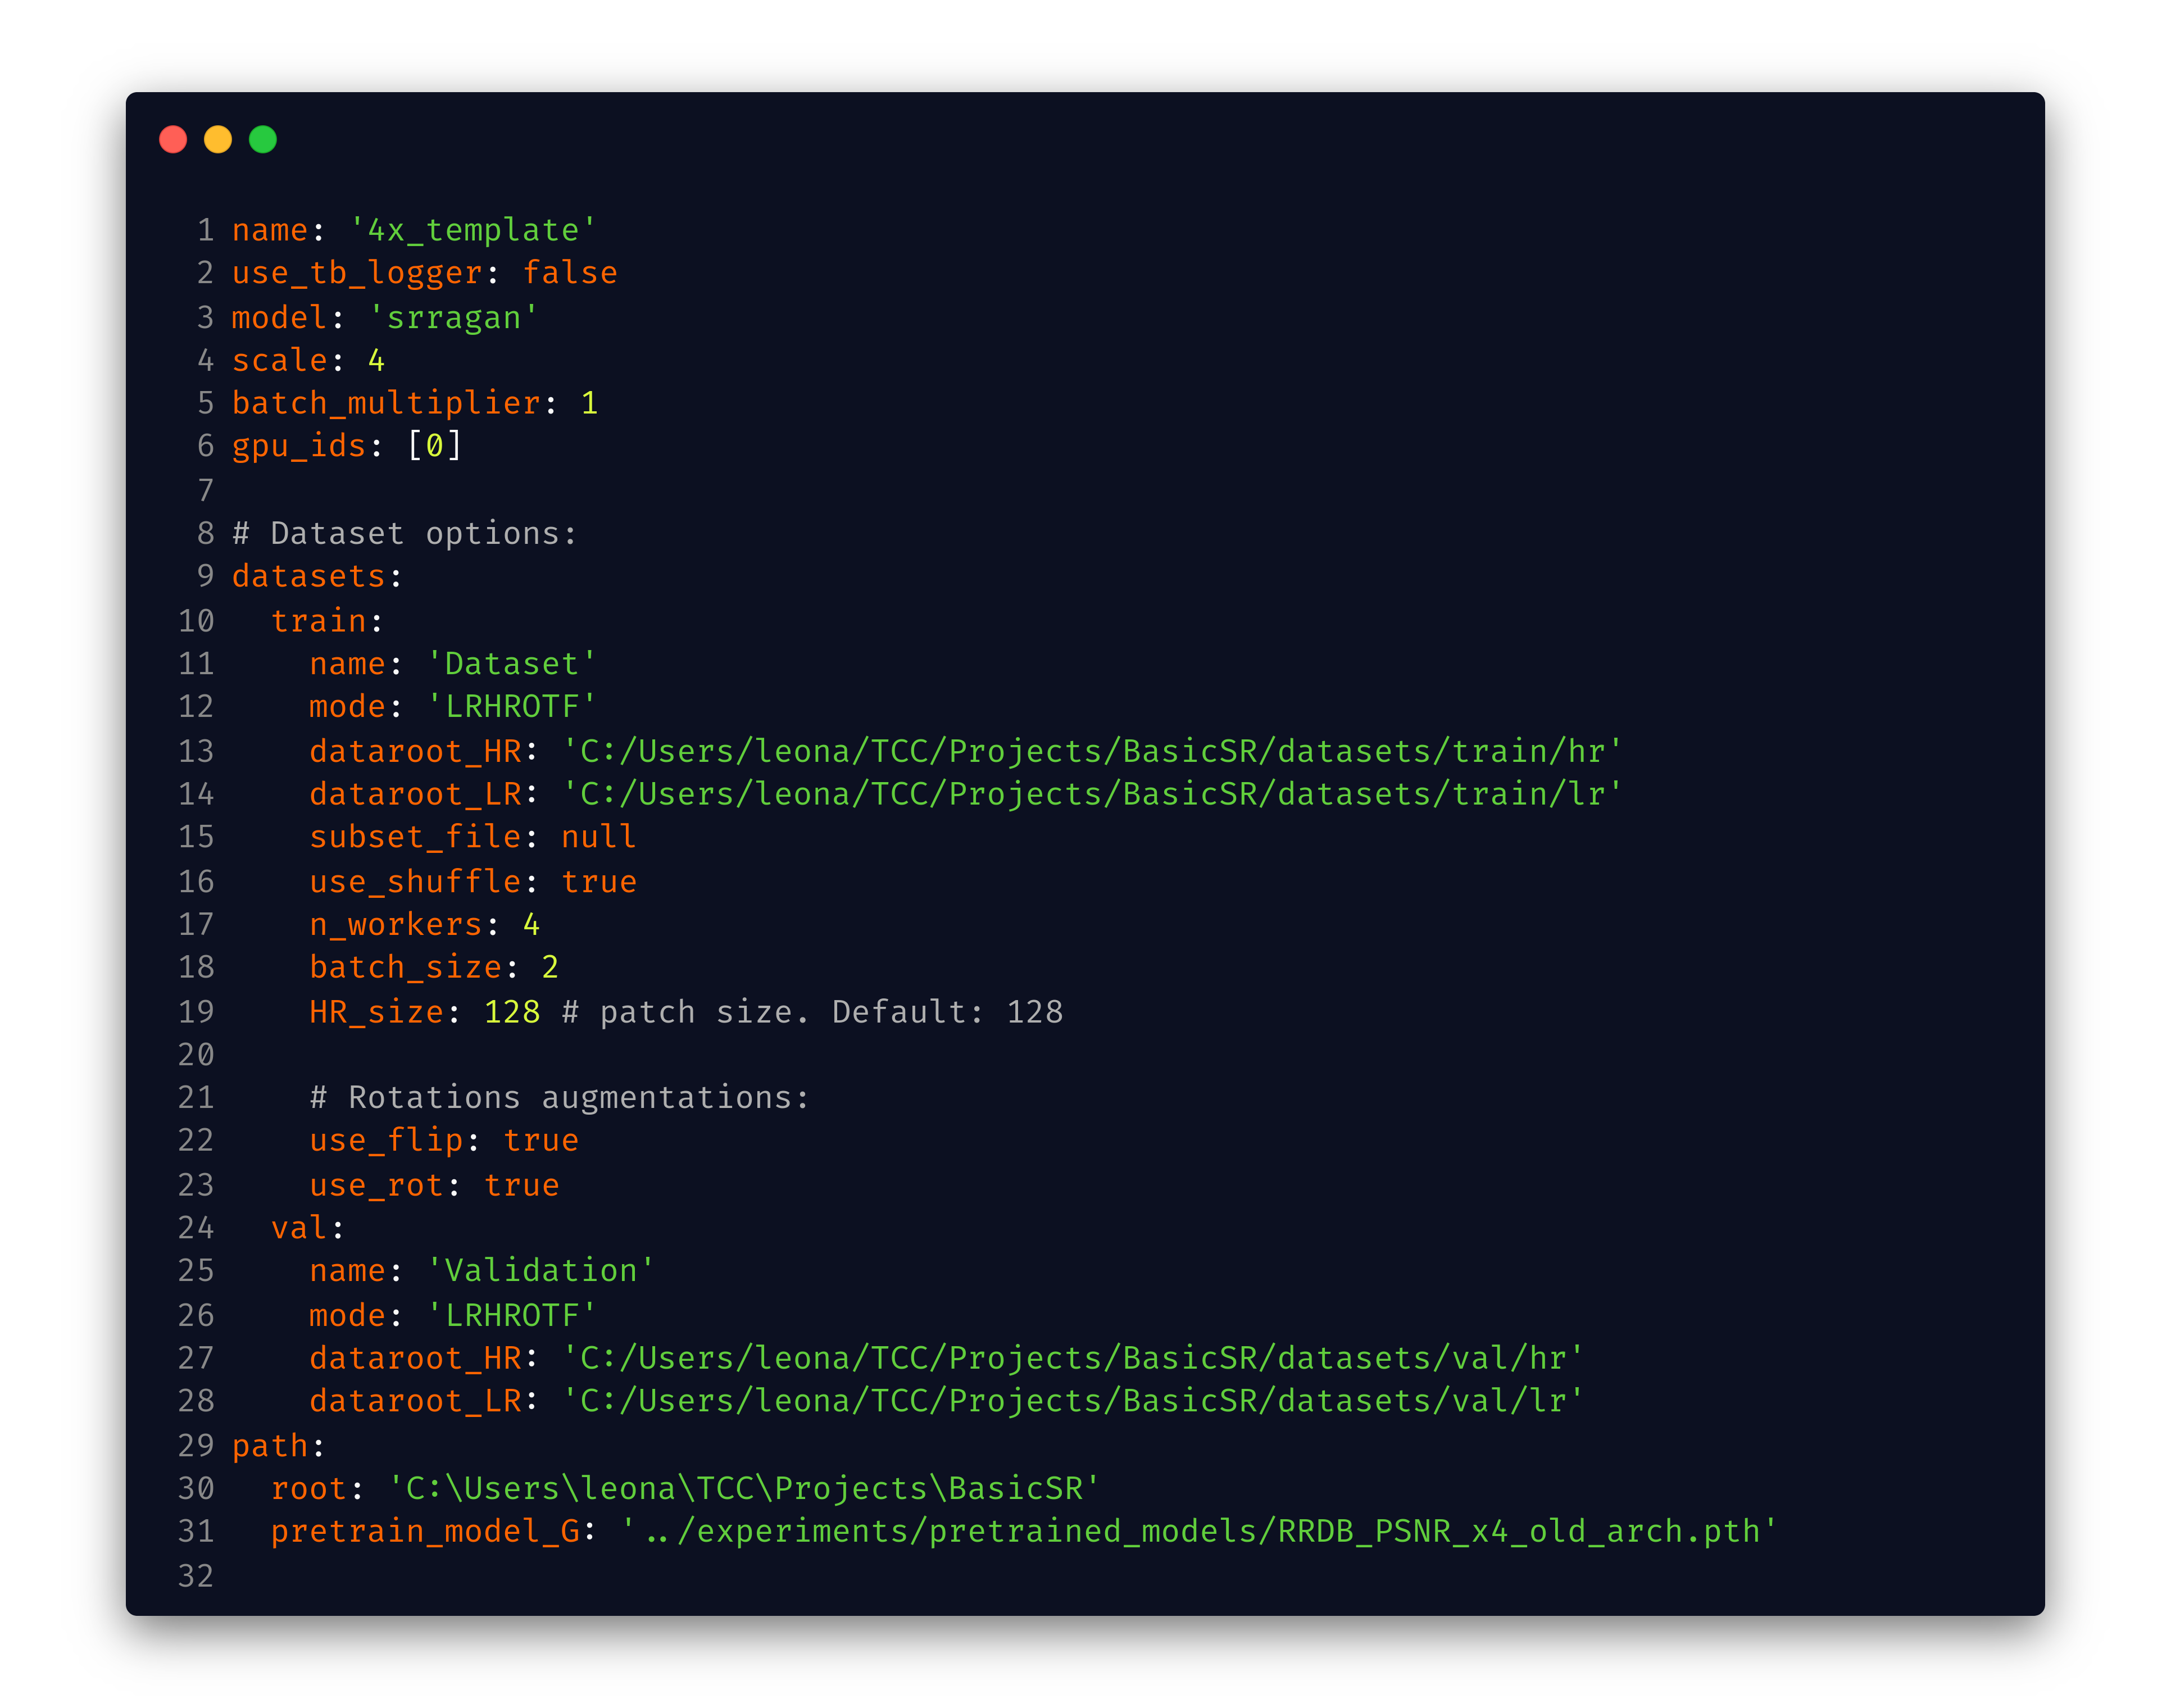
\includegraphics[width=12cm]{fig/carbon_configuracao_basic_sr.png}
    \legend{Fonte: Autor.}
    \label{fig:fig29}
\end{figure}

No arquivo de configuração mostrado anteriormente, alguns parâmetros devem ter atenção especial. O parâmetro \textit{scale} representa a proporção na qual deseja-se treinar o modelo, quatro nesse caso. Os parâmetros \textit{dataroot\_HR} e \textit{dataroot\_LR} representam o diretório com as imagens de alta e baixa resolução, respectivamente, para treino e validação. E por último, mas não menos importante, o atributo \textit{pretrain\_model\_G} é o caminho onde está armazenado o modelo pré-treinado.


\subsection{Descrição dos experimentos práticos de treinamento}

O processo anterior foi feito a partir do zero para duas bases de imagens diferentes, criando uma cópia do projeto no final do processo por segurança. Desta forma, os resultados do modelo terão uma maior reprodutibilidade.

\subsubsection{Executando o modelo}

Com tudo configurado e preparado, basta executar o modelo, com o comando abaixo, seguindo as opções recomendadas na documentação do projeto:

\begin{figure}[H]
    \centering
    \caption{Comando para executar o treinamento.}
    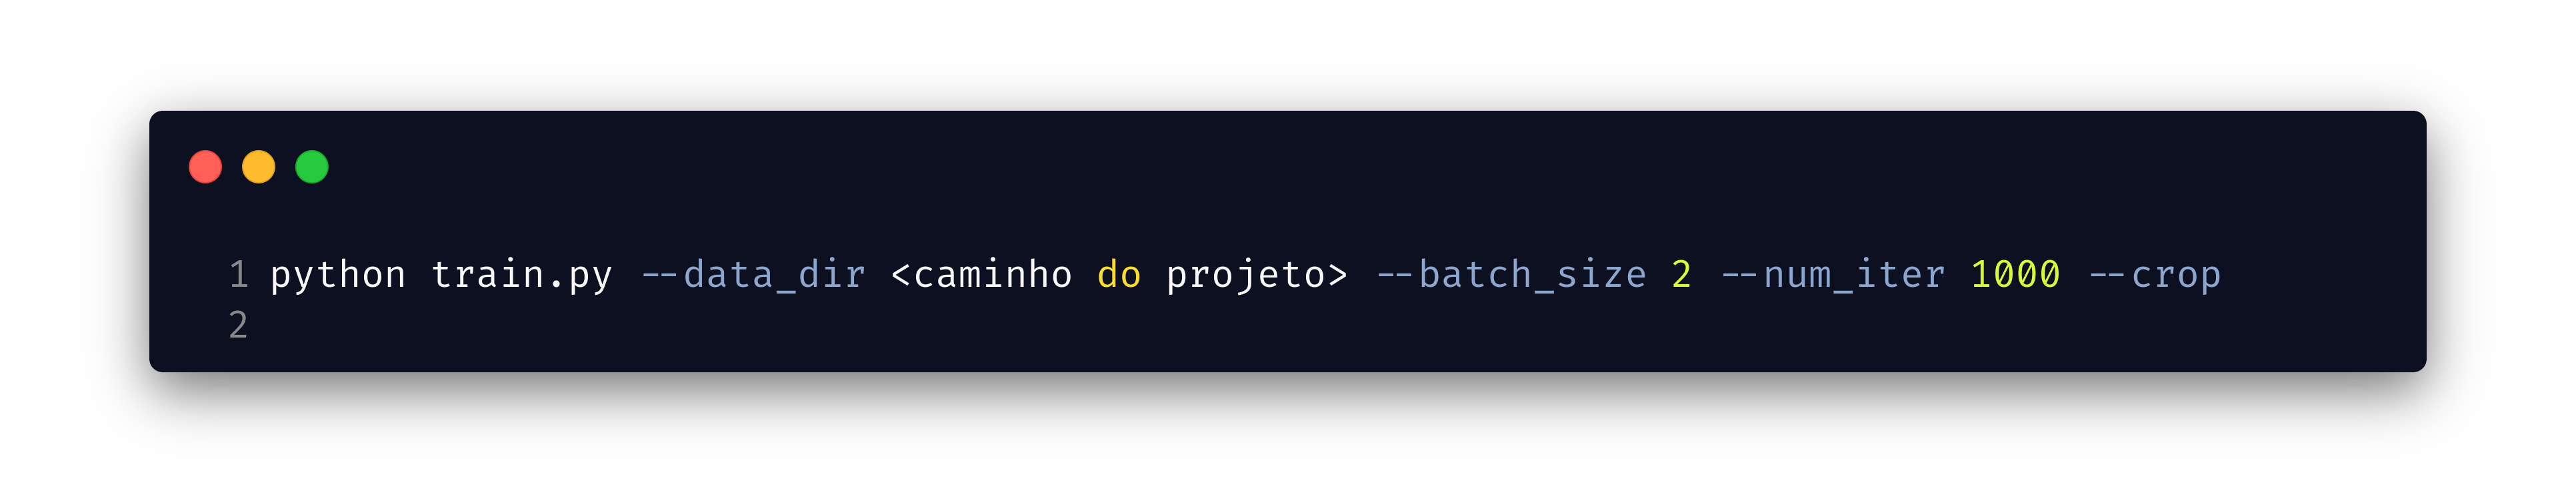
\includegraphics[width=12cm]{fig/carbon_executar_projeto.png}
    \legend{Fonte: Autor.}
    \label{fig:fig30}
\end{figure}

Estes parâmetros utilizados acima, foram os que funcionaram melhor após experimentar com o modelo. Perceba, que o \textit{batch\_size} é 2, assim como no projeto em Tensorflow mencionado anteriormente. No caso anterior, treinar com apenas duas imagens por vez era um impeditivo, dada a extensão no tempo total do treinamento. Com este modelo atual no entanto, em cerca de dez horas o treinamento cobria próximo de 100 épocas com 1000 iterações cada. Um número razoável para o propósito do trabalho. 


\section{Coleta de dados}

Nesta seção, será descrito o procedimento pelo qual a colheita de dados foi feita. Diversas automações foram feitas para extrair o máximo de dados com o mínimo de tempo. Quanto mais dados coletados, mais rica é a analise.

\subsection{Experimentos de similaridade entre imagens}
\label{sec:experimentos-similaridade-imagens}

Como dito na seção \ref{sec:qualidade-imagem}, existem formas quantitativas de avaliar a qualidade de imagens. Um pequeno programa foi desenvolvido para lidar com essa tarefa de forma automatizada \cite{vasconcelos_leonamtvimage-similarity-scripts_2023}. O programa executa em linha de comando, recebendo como parâmetros as duas imagens e os algoritmos de similaridade que será utilizado. O software tem os seguintes algoritmos de similaridade disponíveis: MSE, RMSE, PSNR, UQI, SSIM, ERGAS, SCC, RASE, SAM, MSSSIM e VIFP.

Para o escopo deste trabalho, serão utilizados os algoritmos MSE, RMSE, PSNR e ERGAS. A sintaxe utilizada segue o seguinte padrão

\begin{figure}[H]
    \centering
    \caption{Diagrama de sintaxe do programa.}
    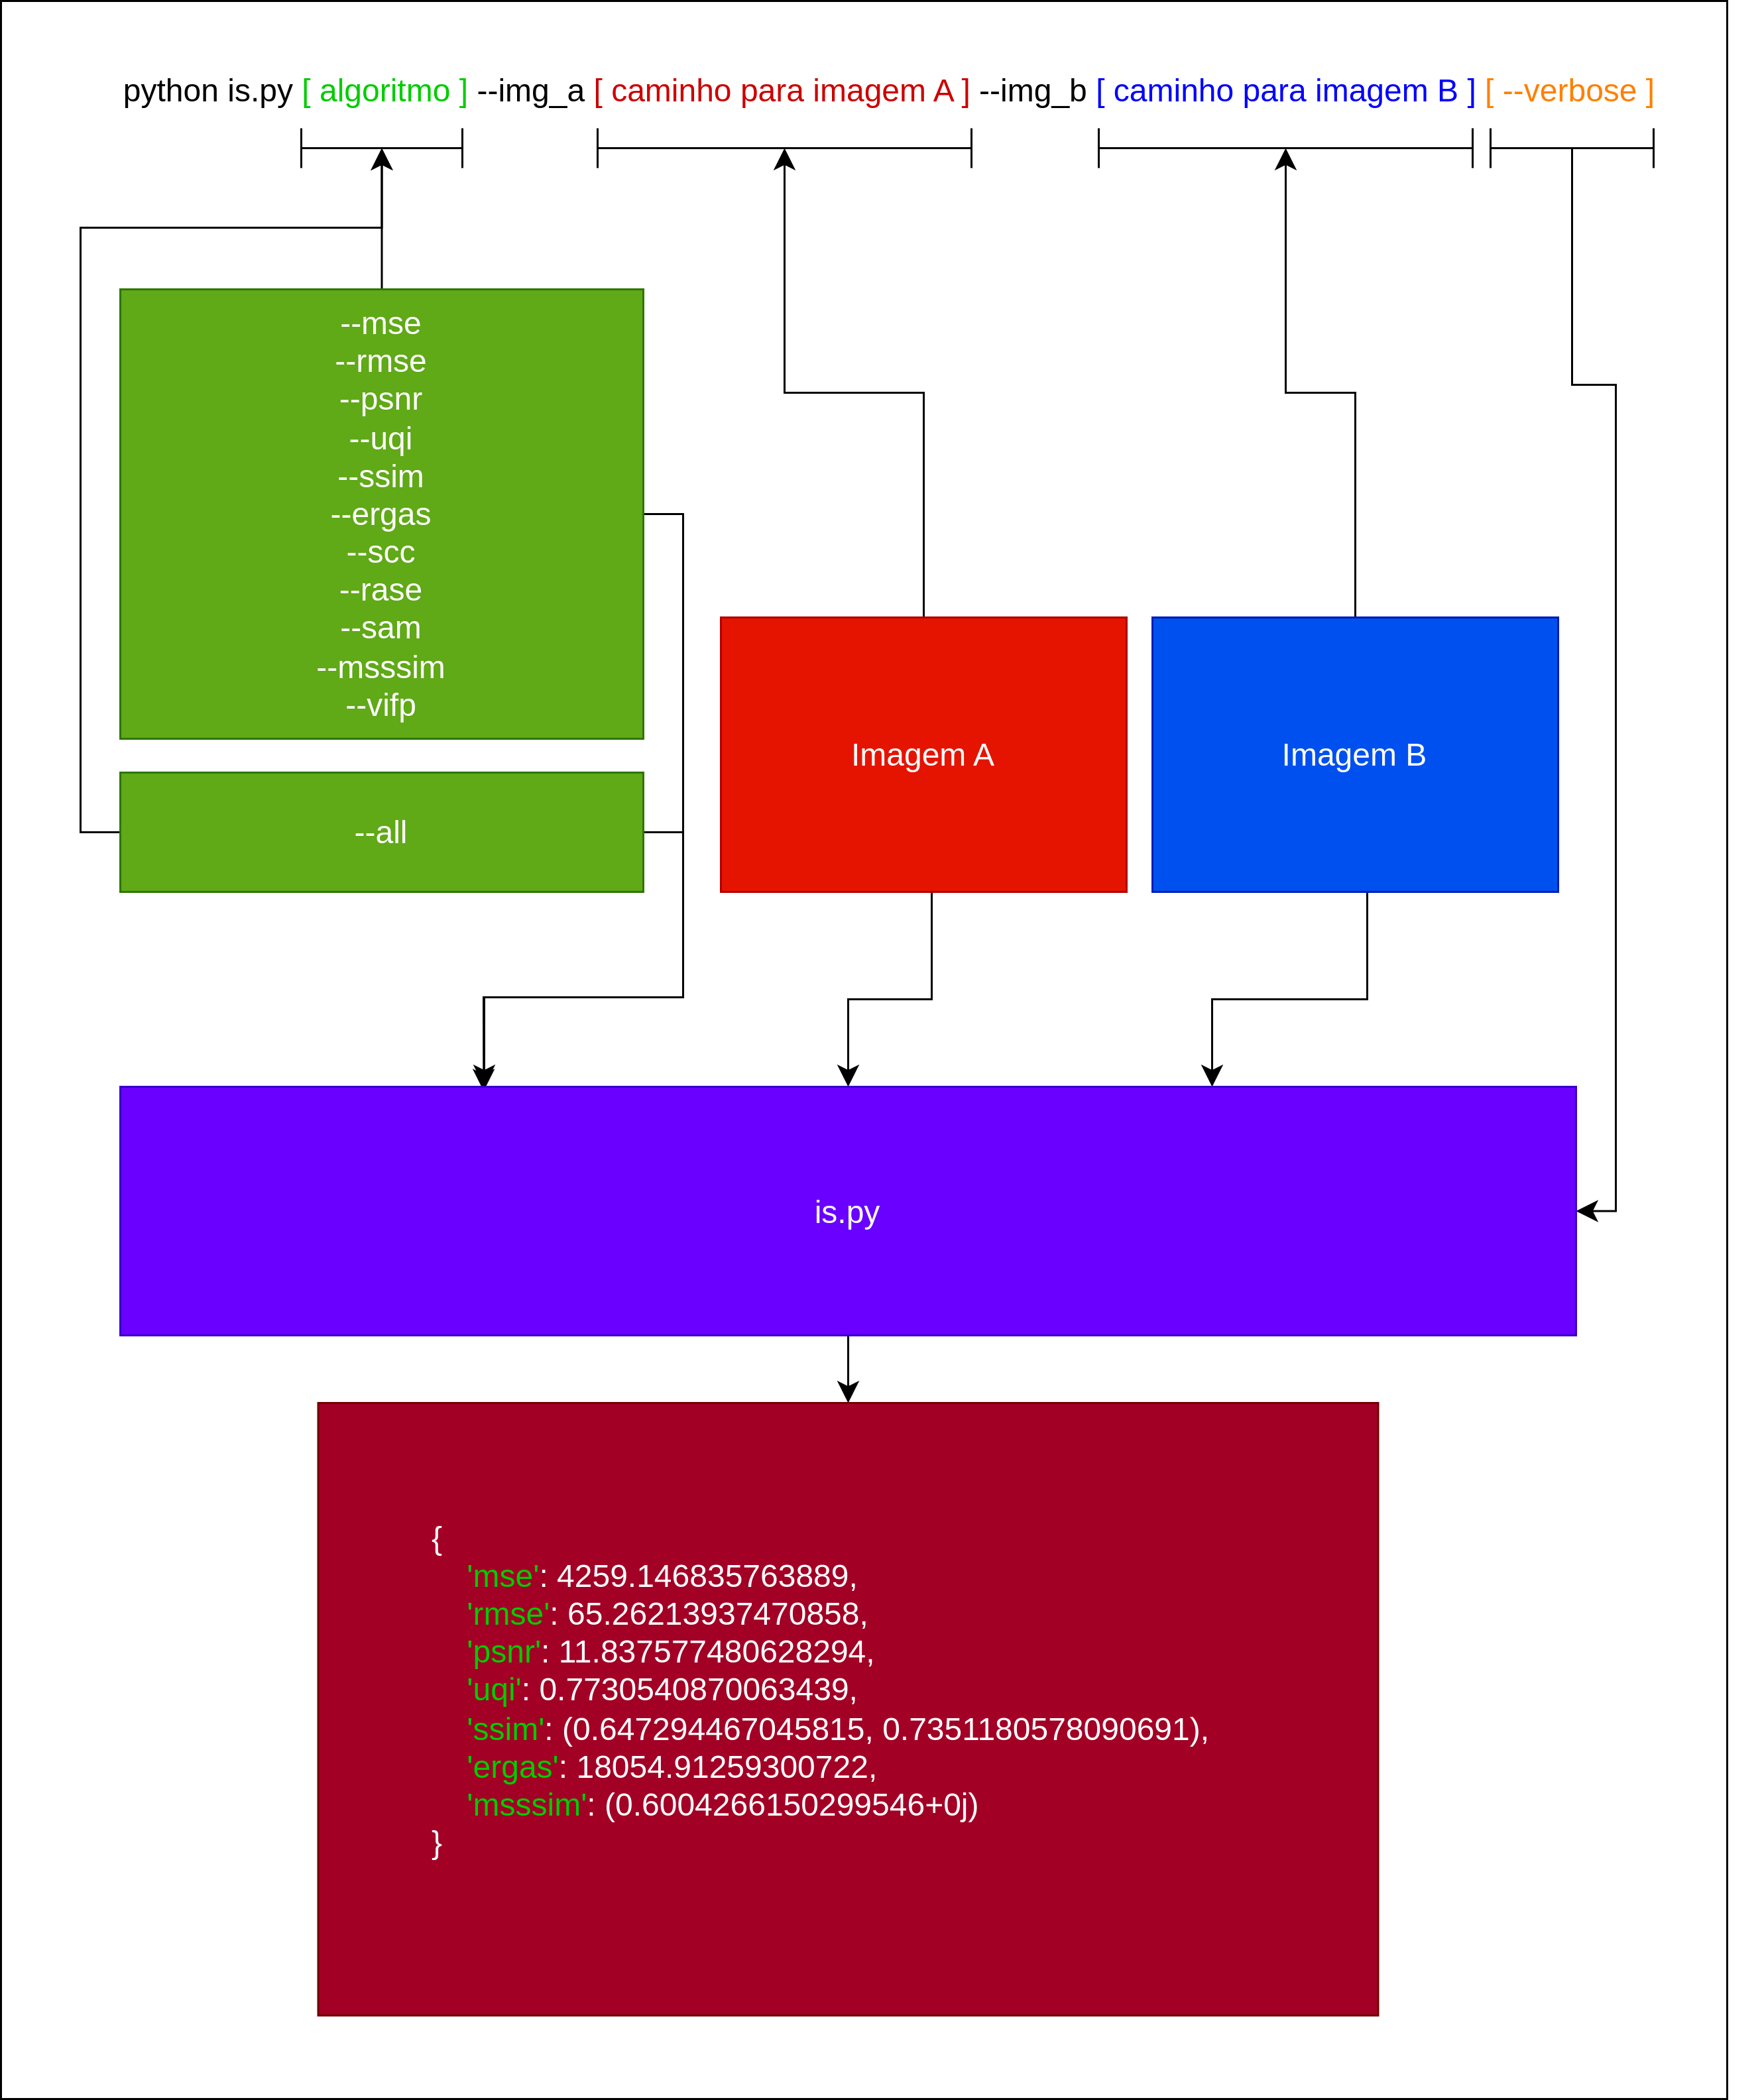
\includegraphics[width=14cm]{fig/similarity/image_similarity_script.png}
    \legend{Fonte: Autor.}
    \label{fig:fig31}
\end{figure}

Na figura \ref{fig:fig31}, o parâmetro \textit{algoritmo} representa quais algoritmos serão utilizados para calcular a similaridade entre as imagens. para executar todos os algoritmos, deve-se passar uma lista com todos os desejados, ou passar o parâmetro \textit{--all}.

Para alimentar o programa com as imagens, os parâmetros \textit{--img\_a} e \textit{--img\_b} são utilizados. Estes recebem os caminhos das imagens. O parâmetro \textit{--verbose}, caso passado, imprime algumas informações a mais.

\subsubsection{Exemplo de execução do programa acima}

Para o exemplo, as duas imagens abaixo serão utilizadas:

\begin{figure}[H]
    \centering
    \caption{Imagem A e imagem B utilizadas no teste.}
    \includegraphics[width=14cm]{fig/similarity/image_a_and_image_b.png}
    \legend{Fonte: Autor (imagens e montagem).}
    \label{fig:fig32}
\end{figure}

Ao se executar o programa nas imagens da figura \ref{fig:fig32}, o resultado demonstrado na tabela \ref{tab:image_similarity_test} é obtido.

\begin{table}[H]
    \centering
    \caption{Tabela de resultados da execução do programa.}
    \begin{tabular}{|l|l|} \hline
        \textbf{Algoritmo} & \textbf{Resultado}      \\ \hline
        MSE                & 4259,146835763889       \\ \hline
        RMSE               & 65,26213937470858       \\ \hline
        PSNR               & 11,837577480628294      \\ \hline
        ERGAS              & 18054,91259300722       \\ \hline
    \end{tabular}
    \vspace{0.3cm}
    \legend{Fonte: Autor.}
    \label{tab:image_similarity_test}
\end{table}

Fazendo uma breve interpretação dos resultados, podemos concluir que a similaridade entre as imagens, como é de se esperar é baixa. A tabela \ref{tab:image_similarity_test_results_analysis}, descreve os resultados.

\begin{table}[H]
    \centering
    \caption{Tabela de descrição dos resultados da execução do programa.}
    \begin{tabular}{|l|l|l|} \hline
        \textbf{Algoritmo} & \textbf{Resultado} & \textbf{Análise}                        \\ \hline
        MSE                & 4259,146835763889  & Quanto mais próximo de 0, mais similar. \\ \hline
        RMSE               & 65,26213937470858  & Quanto mais próximo de 0, mais similar. \\ \hline
        PSNR               & 11,837577480628294 & Quanto maior o valor, mais similar.     \\ \hline
        ERGAS              & 18054,91259300722  & Quanto mais próximo de 0, mais similar. \\ \hline
    \end{tabular}
    \vspace{0.3cm}
    \legend{Fonte: Autor.}
    \label{tab:image_similarity_test_results_analysis}
\end{table}

Agora, apenas como meio de comparação, o programa será executado comparando agora, a imagem A com ela mesma. Os resultados estão na tabela \ref{tab:image_similarity_test_same_image}. 

\begin{table}[H]
    \centering
    \caption{Tabela de resultados da execução do programa com apenas a imagem A.}
    \begin{tabular}{|l|l|} \hline
        \textbf{Algoritmo} & \textbf{Resultado} \\ \hline
        MSE                & 0,0                \\ \hline
        RMSE               & 0,0                \\ \hline
        PSNR               & $\infty$           \\ \hline
        ERGAS              & 0,0                \\ \hline
    \end{tabular}
    \vspace{0.3cm}
    \legend{Fonte: Autor.}
    \label{tab:image_similarity_test_same_image}
\end{table}

\subsection{Coleta das imagens para avaliação dos resultados}

O treinamento das redes adversárias geradoras, produz algumas imagens com as quais o próprio programa de treinamento avalia a performance do modelo. No entanto, a quantidade de imagens produzidas durante o treinamento não é significativa para propriamente se avaliar como o modelo evoluiu após o treinamento.

Para coletar uma quantidade considerável de imagens, basta alimentar o modelo já treinado e armazenar a imagem resultante. No modelo utilizado, é necessário organizar as imagens desejadas em um diretório específico, obedecendo obviamente a estrutura requerida e preencher, com o caminho do diretório, o arquivo de configuração.


\subsubsection{Bases de dados utilizadas para a coleta de dados}

\begin{itemize}
    \item Base de dados médica \ref{sec:imagens_medicas}
    \item Base de dados astronômica \ref{sec:imagens_astronomicas}
\end{itemize}

\subsubsection{Programa para extração de estatísticas das imagens}
\label{sec:programa-extracao-estatisticas-imagem}

O processo de alimentar uma imagem em resolução reduzida à rede já treinada para em seguida formalmente compará-la, utilizando-se dos métodos de similaridade apresentados anteriormente (\ref{sec:qualidade-imagem}) à sua versão original é tedioso e mecânico: características comuns em tarefas automatizáveis.

Para tornar o processo mais eficiente, um programa codificado em \textit{Python} foi implementado. O programa, de forma superficial realiza as seguintes tarefas:

\begin{enumerate}
    \item De um arquivo de configuração, lê uma lista de bases de dados contendo as seguintes informações sobre cada:
    \begin{itemize}
        \item Nome
        \item Caminho do diretório contento os arquivos originais (imagens em alta resolução)
        \item Caminho do diretório contendo os arquivos extraídos da RAG (as mesmas imagens acima, com resoluções reduzidas e alimentadas à RAG)
        \item Extensão dos arquivos
    \end{itemize}
    \item Para cada uma das bases de dados, o programa:
    \begin{itemize}
        \item Lê as imagens do diretório com as imagens já passadas pela RAG
        \item Encontra a imagem equivalente no diretório contendo as imagens originais
        \item Como as imagens originais podem ter dimensões levemente diferentes das imagens que saem da RAG, o programa redimensiona a maior entre as duas imagens, para as dimensões da menor.
        \item Utilizando a biblioteca mencionada na seção \ref{sec:experimentos-similaridade-imagens}, produz um objeto contendo as estatísticas para todas as imagens contidas nos diretórios da configuração.
        \item Salva o objeto como um arquivo \textit{JSON}
    \end{itemize}
\end{enumerate}

\subsubsection{Análise dos resultados}

Uma ferramenta renomada no meio de análise e processamento de dados, é o \textit{Jupyter Notebook}. A ferramenta, consiste em um servidor, provedor de um interpretador interativo no navegador. Este interpretador, fornece de forma direta e eficaz um método para executar várias vezes seguidas, trechos de código, sem precisar de executar novamente o programa inteiro.

A ferramenta é perfeita para a análise dos dados produzidos na seção \ref{sec:programa-extracao-estatisticas-imagem}. Com os arquivos \textit{JSON} em mãos, um para a base de dados de ressonância magnética e outro para a base de dados astronômica, é possível extrair destes os dados e assim criar visualizações para análise dos resultados.


